%% CoPiT manuscript for Computer Physics Communications (CPC)
%% Working directory: /home/ycfan/fyc/paper/copit_paper_2
\documentclass[final,3p,times]{elsarticle}

%% Mathematics and tables
\usepackage{amssymb,amsmath,amsthm}
\usepackage{graphicx}
\usepackage{booktabs}
\usepackage{multirow}
\usepackage{array}
\usepackage{bm}
\usepackage{xcolor}
\usepackage{url}
\usepackage{microtype}
\usepackage{enumitem}

%% Multipanel figures and captions (journal style)
\usepackage{subcaption}
\usepackage[font=small,labelfont=bf,labelsep=period,
            justification=justified,singlelinecheck=false]{caption}
\captionsetup[subfigure]{font=footnotesize,labelfont=bf}

%% Float control (do NOT use placeins[section]: it forces a float flush at
%% every \section and can look like section page breaks when many figures remain)
\usepackage{float}
\usepackage{placeins}

%% Hyperlinks without coloured boxes
\usepackage[hidelinks]{hyperref}

%% Placement parameters (Elsevier / Q1 single-column density)
\renewcommand{\topfraction}{0.85}
\renewcommand{\bottomfraction}{0.70}
\renewcommand{\textfraction}{0.15}
\renewcommand{\floatpagefraction}{0.85}
\renewcommand{\dblfloatpagefraction}{0.85}
\setcounter{topnumber}{3}
\setcounter{bottomnumber}{2}
\setcounter{totalnumber}{5}
\setlength{\textfloatsep}{12pt plus 2pt minus 3pt}
\setlength{\floatsep}{10pt plus 2pt minus 2pt}
\setlength{\intextsep}{10pt plus 2pt minus 2pt}
\setlength{\abovecaptionskip}{5pt}
\setlength{\belowcaptionskip}{3pt}

\newtheorem{proposition}{Proposition}

\journal{Computer Physics Communications}

\begin{document}

\begin{frontmatter}

\title{CoPiT: A conditional position-induced Transformer for aerodynamic field prediction on irregular meshes}

%% TODO: confirm spelling of the student name with the author before submission.
\author[a]{Y.\ Fan\corref{cor1}}
\ead{y.fan@connect.polyu.hk}  % TODO: confirm PolyU email
%% \author[a]{Zhonghua Qiao}
%% \ead{zhonghua.qiao@polyu.edu.hk}

\cortext[cor1]{Corresponding author.}
\address[a]{Department of Applied Mathematics, The Hong Kong Polytechnic University, Hung Hom, Kowloon, Hong Kong, China}

\begin{abstract}
High-fidelity Reynolds-averaged Navier--Stokes (RANS) simulations remain expensive for many-query aerodynamic design. Neural operators offer a mesh-flexible surrogate, yet on irregular aerodynamic data freestream and design parameters are often supplied only by input concatenation, so geometry-driven aggregation and parametric dependence are not cleanly separated. We propose CoPiT (\textbf{Co}nditional \textbf{P}osition-induced \textbf{T}ransformer), which retains a position-induced Transformer (PiT) backbone for geometry-aware interaction on unstructured meshes and injects multi-stage FiLM conditioning from a global parameter vector. FiLM is applied after instance normalisation in each processor block and in the decoder; as a pointwise affine map it does not alter the mesh kernel of position attention and therefore inherits the discretisation-consistency property of PiT. On AirfRANS, under the official full-data, scarce-data and extrapolation protocols, CoPiT attains competitive or best surface and volume field losses among the compared models and substantially improves drag rank correlation relative to graph baselines and Transolver, while using about four times fewer parameters than Transolver. On BlendedNet++, under a unified reimplementation of the forward surface-regression task, CoPiT achieves the lowest overall normalised surface MSE among the tested baselines, with the largest gains on $C_p$ and $C_{f,x}$.
\end{abstract}

\begin{keyword}
neural operator \sep aerodynamic surrogate \sep transformer \sep Feature-wise Linear Modulation
\end{keyword}

\end{frontmatter}

%% PROGRAM SUMMARY temporarily omitted (to be restored for CPiP / program-library submission).

%% =====================================================================
\section{Introduction}
\label{sec:intro}
%% =====================================================================
Parametric partial differential equations (PDEs) are central to fluid mechanics and aerospace applications~\cite{anderson2017fundamentals,vinuesa2022cfd_ml}. In particular, high-fidelity Reynolds-averaged Navier--Stokes (RANS) simulations yield velocity, pressure and wall-shear fields that are indispensable for aerodynamic analysis, yet each solve is computationally expensive. Many-query tasks---design exploration, optimisation and multi-condition evaluation---therefore motivate surrogate models that approximate the map from geometry and freestream or design parameters to aerodynamic fields at a fraction of the CFD cost~\cite{brunton2020ml_fluid,karniadakis2021piml}. Figure~\ref{fig:surrogate_pipeline} illustrates this surrogate-assisted workflow.

\begin{figure}[!htbp]
\centering
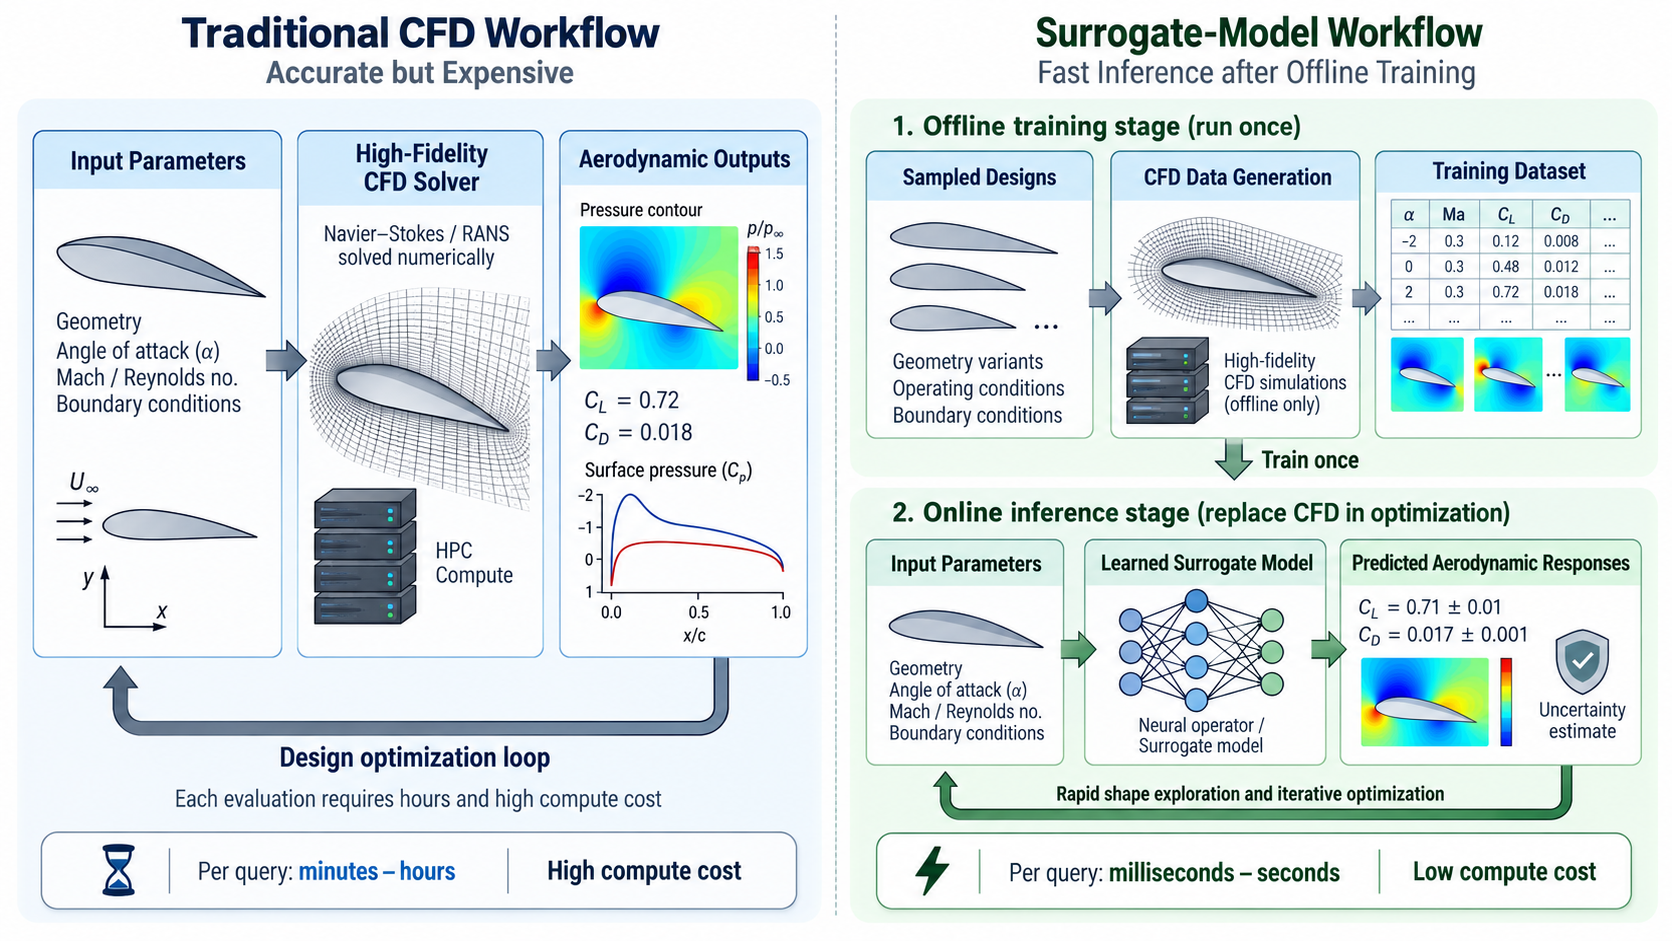
\includegraphics[width=0.92\linewidth,height=0.27\textheight,keepaspectratio]{figs/fig1_v2.png}
\caption{Surrogate-assisted aerodynamic design workflow. A learned surrogate approximates the CFD solution operator, replacing repeated high-cost RANS evaluations with fast inference during iterative design exploration and optimisation.}
\label{fig:surrogate_pipeline}
\end{figure}

Neural operators learn mappings between function spaces and, once trained, evaluate new inputs by a single forward pass~\cite{li2021fno,lu2021deeponet,kovachki2023neural}. Fourier Neural Operators (FNO) and DeepONet are standard constructions on structured domains~\cite{li2021fno,lu2021deeponet}; Geo-FNO and GINO extend related ideas to more general geometries~\cite{li2023geofno,li2022gino}. Graph networks and transformer-based solvers further address unstructured meshes~\cite{pfaff2021learning,wu2024transolver,luo2025transolverpp,chen2024pit}. These developments make operator learning a natural framework for aerodynamic field prediction, where the surrogate must remain accurate across varying meshes and parametric regimes.

Aerodynamic data differ from many PDE benchmarks in two respects. First, the discrete domain is geometry-dependent (unstructured meshes or surface triangulations) rather than a fixed Cartesian grid. Second, the solution depends jointly on local geometry and global parameters such as freestream speed, angle of attack and design variables~\cite{bhatnagar2019cnn_aero,thuerey2020deepcfd,bonnet2022airfrans,sung2025blendednetpp}. Geometry-aware architectures (MeshGraphNets, Transolver, PiT) capture spatial interactions effectively~\cite{pfaff2021learning,wu2024transolver,chen2024pit}, but freestream and design parameters are often supplied only by input concatenation and then processed only implicitly by the backbone. Such one-shot fusion mixes geometry-driven aggregation with parametric response modulation and can reduce sensitivity to those parameters in deeper layers---a limitation that is especially relevant when integrated forces must be ranked across flight regimes.

Feature-wise Linear Modulation (FiLM) offers a lightweight alternative: a small network maps a parameter vector to channel-wise scale and shift coefficients that modulate intermediate features~\cite{perez2018film,dumoulin2018film_survey}. Originally developed for visual reasoning, FiLM is adopted here as an explicit, multi-stage conditioning mechanism inside a mesh-based operator.

We propose \emph{CoPiT}, a \textbf{Co}nditional \textbf{P}osition-induced \textbf{T}ransformer for aerodynamic field prediction. CoPiT retains PiT---position-induced attention with a latent-mesh encode--process--decode structure~\cite{chen2024pit}---as the geometric backbone, and injects multi-stage FiLM conditioning after instance normalisation in every processor block and in the decoder. Geometric interactions remain positional; freestream and design parameters act through depth-wise affine modulation. We evaluate CoPiT on AirfRANS~\cite{bonnet2022airfrans} (two-dimensional RANS airfoil fields; full, scarce and extrapolation protocols) and on BlendedNet++~\cite{sung2025blendednetpp} (three-dimensional blended-wing-body surface fields).

The contributions of this work are as follows:
\begin{itemize}[leftmargin=1.4em,itemsep=0.2em,topsep=0.3em]
\item \textbf{Architecture.} We propose CoPiT, which couples a PiT geometric backbone with multi-stage FiLM so that mesh-based aggregation and parametric modulation are handled by distinct components rather than by input concatenation alone.
\item \textbf{Analysis.} FiLM acts as a pointwise affine map on features and therefore leaves the positional attention kernel unchanged, so CoPiT inherits the discretisation-consistency property of PiT.
\item \textbf{Experiments.} We provide a systematic evaluation on AirfRANS and BlendedNet++, including comparisons with graph and transformer baselines under matched protocols.
\end{itemize}

The remainder of the paper is organised as follows. Section~\ref{sec:prelim} states the learning problem and reviews position-induced attention and the PiT backbone. Section~\ref{sec:method} introduces CoPiT. Section~\ref{sec:experiments} reports numerical experiments. Section~\ref{sec:conclusion} concludes.


%% =====================================================================
\section{Preliminaries}
\label{sec:prelim}
%% =====================================================================
We first state the operator-learning setting and then summarise position-induced attention as developed for the Position-induced Transformer (PiT)~\cite{chen2024pit}.

\subsection{Operator learning}
\label{sec:op_learn}
Consider a parametric PDE of the form
\begin{equation}
  \mathcal{L}_{a}u = f,
  \label{eq:pde}
\end{equation}
where
\begin{equation}
  a \in \mathcal{A}(\Omega_{a};\mathbb{R}^{d_{a}}),
  \qquad
  u \in \mathcal{U}(\Omega_{u};\mathbb{R}^{d_{u}}),
  \qquad
  f \in \mathcal{F}.
  \label{eq:spaces}
\end{equation}
Here $\Omega_{a},\Omega_{u}\subset\mathbb{R}^{d}$ are bounded domains (not necessarily identical), $\mathcal{A}$ and $\mathcal{U}$ are Banach spaces of functions over $\Omega_{a}$ and $\Omega_{u}$, respectively, and $\mathcal{L}_{a}:\mathcal{U}\to\mathcal{F}$ is a differential operator depending on the parameter function $a$. The associated solution operator is
\begin{equation}
  \Phi : \mathcal{A} \to \mathcal{U},
  \qquad
  u = \Phi(a).
  \label{eq:solution_op}
\end{equation}
Operator learning aims to construct a parameterised surrogate $\Phi_{\theta}$ such that $\Phi_{\theta}(a)\approx\Phi(a)$ for previously unseen inputs $a$~\cite{kovachki2023neural,li2021fno,chen2024pit}.

In applications, $a$ and $u$ are observed only through samples on finite meshes
\begin{equation}
  X_{a}
  =
  \{x_{i}\}_{i=1}^{N_{a}}
  \subset
  \Omega_{a},
  \qquad
  X_{u}
  =
  \{\hat{x}_{i}\}_{i=1}^{N_{u}}
  \subset
  \Omega_{u}.
  \label{eq:meshes}
\end{equation}
Given training pairs $\{(a^{j},u^{j})\}_{j=1}^{J}$, with $a^{j}$ sampled on $X_{a}$ and $u^{j}$ on $X_{u}$, the parameters $\theta$ are obtained by minimising
\begin{equation}
  \min_{\theta}\;
  \frac{1}{J}
  \sum_{j=1}^{J}
  \bigl\|
    u^{j}
    -
    \Phi_{\theta}(a^{j})
  \bigr\|^{2},
  \label{eq:emp_risk}
\end{equation}
where the residual is evaluated on the output mesh (or on a subsample of it). After training, $\Phi_{\theta}$ is expected to accept new sampling locations of $a$ and to predict $u$ at arbitrary query locations in $\Omega_{u}$.

\noindent\textbf{Aerodynamic setting.}\ 
In the present work the parameter function is induced by a geometry $g$ and a global parameter vector $\mathbf{c}\in\mathbb{R}^{d_{c}}$ collecting freestream and design quantities. We write $a=a_{g,\mathbf{c}}$ and allow $\Omega_{a}$ and $\Omega_{u}$ to depend on $g$. The output fields considered later are
\begin{align}
  u_{g,\mathbf{c}}(x)
  &=
  \bigl(v_{x}(x),\, v_{y}(x),\, p(x),\, \nu_{t}(x)\bigr)
  &&
  \text{(AirfRANS)},
  \label{eq:airfrans_target}\\
  u_{g,\mathbf{c}}(x)
  &=
  \bigl(C_{p}(x),\, C_{f,x}(x),\, C_{f,y}(x),\, C_{f,z}(x)\bigr)
  &&
  \text{(BlendedNet++)},
  \label{eq:bwb_target}
\end{align}
and the learning task is to approximate $u_{g,\mathbf{c}}$ by $\Phi_{\theta}(a_{g,\mathbf{c}})$ under the corresponding data protocol.

\subsection{Position-induced attention}
\label{sec:posatt}
A standard building block of Transformer architectures is content-based self-attention~\cite{vaswani2017attention}. Given a feature matrix $U\in\mathbb{R}^{N\times d}$ and trainable matrices $W^{Q}$, $W^{K}$ and $W^{V}$,
\begin{equation}
  \operatorname{SelfAtt}(U)
  =
  \operatorname{Softmax}
  \biggl(
    \frac{U W^{Q}\,(U W^{K})^{\top}}{\sqrt{d}}
  \biggr)
  \, U W^{V}.
  \label{eq:self_att}
\end{equation}
The attention weights depend on feature affinities. Consequently they must be recomputed for every input field, and they do not directly encode the geometry of the underlying mesh. For PDE surrogates this is unnatural: the relative positions of sampling points largely determine how local information should be aggregated.

Position-induced attention incorporates such geometric structure in an explicit and efficient way~\cite{chen2024pit}. Let $U\in\mathbb{R}^{N_{v}\times d_{\ell}}$ collect the values of a feature field on a mesh $X_{v}=\{x_{i}\}_{i=1}^{N_{v}}$, and define the pairwise squared-distance matrix
\begin{equation}
  D_{ij}
  =
  \|x_{i}-x_{j}\|_{2}^{2},
  \qquad
  i,j=1,\ldots,N_{v}.
  \label{eq:dist_mat}
\end{equation}
With a positive bandwidth $\lambda>0$ and a value matrix $W^{V}$, the basic position-attention operator is
\begin{equation}
  \operatorname{PosAtt}(U;D)
  =
  \operatorname{Softmax}(-\lambda D)\,
  U W^{V}.
  \label{eq:posatt}
\end{equation}
Each row of the output is therefore a distance-weighted average of value-transformed features: the kernel depends on mesh geometry rather than on the current feature content. Multi-head variants employ head-wise scales $\lambda_{h}$, implemented through a positive reparameterisation $\phi(\lambda_{h})$. When the query and key meshes differ, the same construction yields \emph{cross} position-attention and realises a learnable change of resolution; when they coincide, one obtains \emph{self} position-attention on a single mesh. A locality parameter $\tau\in(0,1]$ may further restrict attention to a nearest-neighbour fraction of keys (quantile masking), while $\tau=1$ recovers a global kernel.

A central property of~\eqref{eq:posatt} is discretisation consistency: as the underlying mesh is refined, the discrete operator converges in probability to an integral operator with a normalised Gaussian-type kernel. A precise statement and proof are given as Theorem~2.1 in~\cite{chen2024pit}. This property makes position-attention an attractive geometric primitive for mesh-based aerodynamic surrogates.

In the PiT architecture~\cite{chen2024pit}, position-attention is organised in an encoder--processor--decoder form with a latent mesh of moderate size. Cross position-attention maps the input mesh to the latent mesh and, later, the latent representation to the output mesh, while a stack of self position-attention blocks refines features on the latent mesh. The next section builds CoPiT on this geometric organisation.


%% =====================================================================
\section{CoPiT: conditional position-induced Transformer}
\label{sec:method}
%% =====================================================================
Relative to PiT, CoPiT adds multi-stage FiLM generators driven by the global condition $\mathbf{c}$, inserted in the processor and the decoder. Position attention, the latent mesh and the encode--process--decode skeleton follow Section~\ref{sec:prelim}.

\subsection{Overview}
\label{sec:overview}


\begin{figure}[!htbp]
\centering
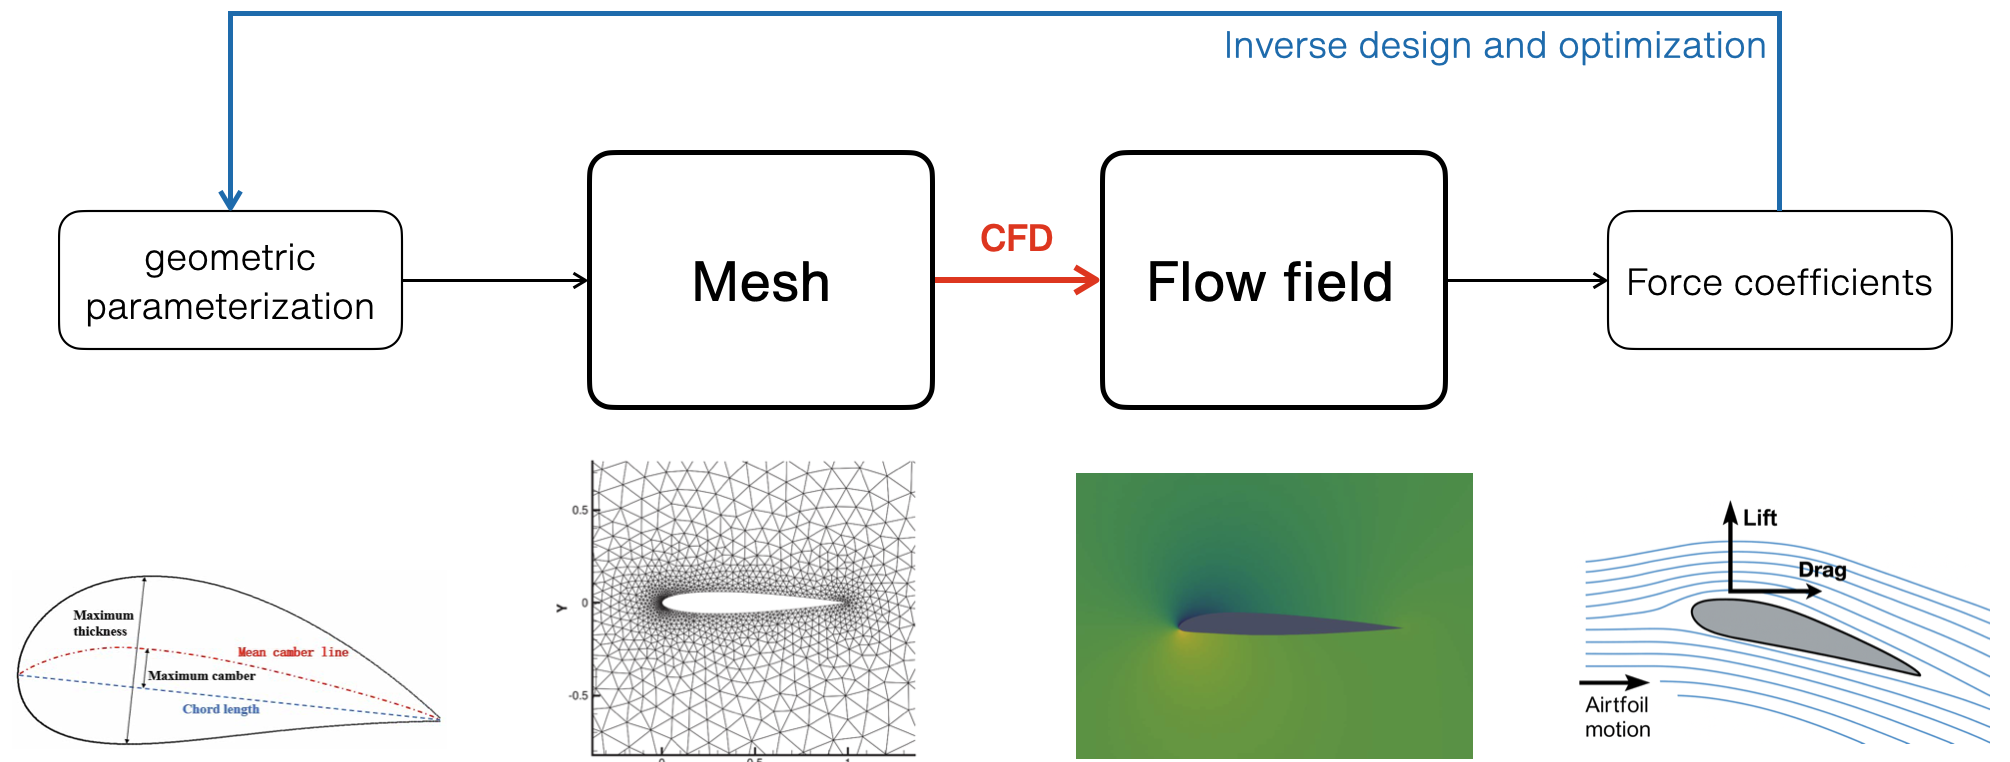
\includegraphics[width=0.92\linewidth,height=0.26\textheight,keepaspectratio]{figs/framework.png}
\caption{Overview of CoPiT: a PiT encode--process--decode backbone with multi-stage FiLM conditioning from the global parameter vector.}
\label{fig:copit_arch}
\end{figure}
Figure~\ref{fig:copit_arch} summarises CoPiT. Given an input mesh with geometric features, a target mesh and a condition vector $\mathbf{c}$, the network (i)~encodes the input onto a latent mesh, (ii)~refines latent features with $L$ processor blocks, each followed by FiLM, and (iii)~decodes to the target mesh with a final FiLM stage before the readout. The same skeleton is used for AirfRANS and BlendedNet++; only dimensions, the content of $\mathbf{c}$ and auxiliary decoder channels change (Section~\ref{sec:instantiate}).

\subsection{Multi-stage FiLM conditioning}
\label{sec:film}


\begin{figure}[!htbp]
\centering
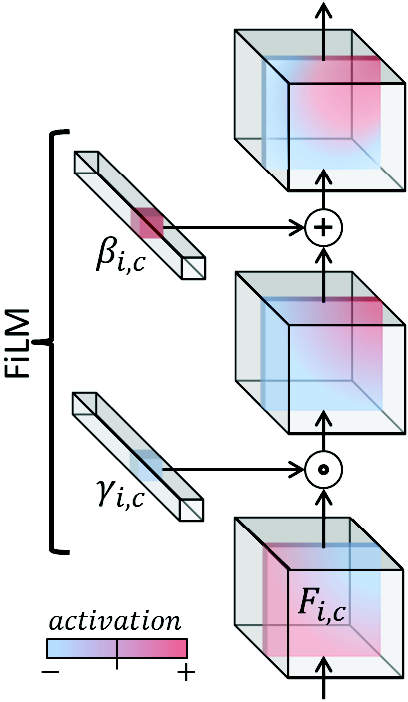
\includegraphics[width=0.32\linewidth,height=0.22\textheight,keepaspectratio]{figs/film.png}
\caption{Feature-wise Linear Modulation (FiLM)~\cite{perez2018film}. A global condition vector produces channel-wise scale $\gamma$ and shift $\beta$, applied as an affine transform to intermediate features.}
\label{fig:film}
\end{figure}
Let $\mathbf{h}\in\mathbb{R}^{D}$ be a hidden feature at a mesh (or latent) point after instance normalisation~\cite{ulyanov2016instance}. A FiLM generator $g_{\theta}:\mathbb{R}^{d_{c}}\to\mathbb{R}^{2D}$ maps $\mathbf{c}$ to scale and shift vectors $(\gamma(\mathbf{c}),\beta(\mathbf{c}))$ and applies
\begin{equation}
  \tilde{\mathbf{h}}
  =
  \gamma(\mathbf{c})\odot\mathbf{h}+\beta(\mathbf{c}).
  \label{eq:film}
\end{equation}
Figure~\ref{fig:film} illustrates the mechanism~\cite{perez2018film}. CoPiT uses two generators:
\begin{itemize}
\item \emph{Processor FiLM}: outputs $\{(\gamma_{\ell},\beta_{\ell})\}_{\ell=1}^{L}$ for all processor blocks (tensor size proportional to $L(1+H)D_{\mathrm{hid}}$);
\item \emph{Decoder FiLM}: outputs $(\gamma_{\mathrm{dec}},\beta_{\mathrm{dec}})$ for the decoder feature map.
\end{itemize}
Each generator is a small MLP (one hidden layer of width $64$ in our experiments) trained end-to-end. Conditions therefore modulate every processing depth rather than only the input layer.

Equation~\eqref{eq:film} implies the following elementary properties of affine channel-wise modulation; the approximation statement is a standard consequence of universal approximation for multilayer perceptrons~\cite{hornik1989mlp}.

\begin{proposition}[Basic properties of FiLM]
\label{prop:film}
Let $\tilde{\mathbf{h}}=\gamma(\mathbf{c})\odot\mathbf{h}+\beta(\mathbf{c})$. Then:
\begin{enumerate}
\item[(i)] $\gamma\equiv\mathbf{1}$ and $\beta\equiv\mathbf{0}$ recover the unmodulated feature;
\item[(ii)] $\gamma_{k}=\beta_{k}=0$ suppresses channel $k$;
\item[(iii)] on any compact set of conditions, continuous maps $\mathbf{c}\mapsto(\gamma(\mathbf{c}),\beta(\mathbf{c}))$ can be approximated uniformly by a feed-forward generator of sufficient width~\cite{hornik1989mlp}.
\end{enumerate}
\end{proposition}

\subsection{Processor and decoder with FiLM}
\label{sec:blocks}
Denote latent features after encoding by $\mathbf{f}_{\mathrm{ltt}}^{(0)}$. Processor block $\ell=1,\ldots,L$ implements
\begin{align}
  \mathbf{h}_{\ell}
  &=
  \mathrm{PosAtt}\bigl(\mathcal{X}_{\mathrm{ltt}},\,\mathbf{f}_{\mathrm{ltt}}^{(\ell-1)}\bigr),
  \label{eq:proc1}\\
  \bar{\mathbf{h}}_{\ell}
  &=
  \mathrm{InstanceNorm}(\mathbf{h}_{\ell}),
  \label{eq:proc2}\\
  \tilde{\mathbf{h}}_{\ell}
  &=
  \gamma_{\ell}(\mathbf{c})\odot\bar{\mathbf{h}}_{\ell}+\beta_{\ell}(\mathbf{c}),
  \label{eq:proc3}\\
  \mathbf{f}_{\mathrm{ltt}}^{(\ell)}
  &=
  \mathbf{f}_{\mathrm{ltt}}^{(\ell-1)}
  +
  \mathrm{GELU}\bigl(\mathrm{MLP}_{\ell}(\tilde{\mathbf{h}}_{\ell})\bigr).
  \label{eq:proc4}
\end{align}
Equation~\eqref{eq:proc3} is the only difference from an unconditioned PiT processor block. The decoder applies position-based cross-attention from $\mathcal{X}_{\mathrm{ltt}}$ to $\mathcal{X}_{\mathrm{out}}$, optionally merges auxiliary channels $\mathbf{a}$ (in particular the signed distance to the wall), then modulates and reads out:
\begin{align}
  \mathbf{g}
  &=
  \mathrm{PosAttCross}\bigl(\mathcal{X}_{\mathrm{out}},\mathcal{X}_{\mathrm{ltt}},\mathbf{f}_{\mathrm{ltt}}^{(L)}\bigr),
  \label{eq:dec1}\\
  \mathbf{g}
  &\leftarrow
  \mathrm{MLP}_{\mathrm{merge}}\bigl([\mathbf{g}\|\mathrm{MLP}_{\mathrm{aux}}(\mathbf{a})]\bigr),
  \label{eq:dec2}\\
  \mathbf{g}
  &\leftarrow
  \gamma_{\mathrm{dec}}(\mathbf{c})\odot\mathrm{InstanceNorm}(\mathbf{g})+\beta_{\mathrm{dec}}(\mathbf{c}),
  \label{eq:dec3}\\
  \hat{\mathbf{u}}_{\mathrm{out}}
  &=
  \mathrm{MLP}_{\mathrm{de}}(\mathbf{g}).
  \label{eq:dec4}
\end{align}
Linear layers use Kaiming initialisation~\cite{he2016resnet} and GELU activations. Residual connections in~\eqref{eq:proc4} stabilise deep processors.

\subsection{Discretisation consistency under FiLM}
\label{sec:consistency}
Position attention converges under mesh refinement to a kernel integral operator~\cite{chen2024pit}. FiLM~\eqref{eq:film} is a pointwise map independent of the mesh connectivity. If $\mathcal{F}_{\lambda}$ denotes the positional attention operator and $\Phi_{\mathbf{c}}$ the affine FiLM map at a fixed condition, then
\begin{equation}
  \bigl\|\Phi_{\mathbf{c}}(\mathcal{F}_{\lambda}(U^{n}))
        -\Phi_{\mathbf{c}}(\mathcal{F}|_{X_{n}})\bigr\|
  \le
  \|\gamma(\mathbf{c})\|_{\infty}\,
  \bigl\|\mathcal{F}_{\lambda}(U^{n})-\mathcal{F}|_{X_{n}}\bigr\|.
  \label{eq:composed_convergence}
\end{equation}
Thus discretisation consistency of the geometric backbone is inherited by CoPiT; FiLM does not introduce mesh-dependent kernels of its own.

\subsection{Task instantiations}
\label{sec:instantiate}
\textbf{AirfRANS.} Spatial dimension $d=2$. In the default configuration used in our experiments, the encoder receives four geometric channels (surface coordinates and unit normals). The freestream state $\mathbf{c}=(U_{\infty},\alpha)$ enters only through the FiLM generators and is not concatenated into the encoder features. The network predicts $(v_{x},v_{y},p,\nu_{t})$ on the CFD mesh. The decoder is conditioned on the signed distance to the wall (SDF) via a small auxiliary MLP that is merged with the cross-attention features before the decoder FiLM and readout. Encoder locality uses $\tau=0.01$; processor self-attention uses $\tau=1$; the decoder employs a smooth (unmasked) position-induced cross-attention projection, which removes the hard quantile cutoff of the original PiT decoder and yields more continuous surface reconstructions.

\textbf{BlendedNet++.} Spatial dimension $d=3$. Pointwise inputs follow an 18-dimensional encoding that includes surface coordinates, normals and broadcast global features; the 12-dimensional design/flight vector $\mathbf{c}$ additionally drives FiLM. The training loss is the mean MSE over $(C_{p},C_{f,x},C_{f,z})$; $C_{f,y}$ is retained for optional evaluation but is not included in the reported training objective. The latent mesh retains 10\% of the surface points by Z-order sampling. Pairwise distances for the official-split experiments use a symmetric geometry-aware metric (\texttt{metric\_sym6}) in place of raw Euclidean distance in ambient $\mathbb{R}^{3}$.


%% =====================================================================
\section{Numerical experiments}
\label{sec:experiments}
We evaluate CoPiT on AirfRANS and BlendedNet++ under standard splits and metrics, and compare against graph and transformer baselines.

\subsection{Experimental setup}
\label{sec:setup}

\subsubsection{Datasets and metrics}
\textbf{AirfRANS}~\cite{bonnet2022airfrans} provides two-dimensional RANS simulations around NACA-family airfoils under freestream states $(U_{\infty},\alpha)$, with unstructured meshes of order $1.8\times 10^{5}$ points. We report surface and volume field losses for $(v_{x},v_{y},p,\nu_{t})$ together with Spearman rank correlations $\rho_{d}$ and $\rho_{l}$ of the drag and lift coefficients. Force coefficients are obtained by surface integration of pressure and wall shear following the AirfRANS protocol (iterative subsampling and PyVista gradients). Four tasks are considered: full data (800/200 train/test), scarce data (200/200), Reynolds-number extrapolation and angle-of-attack extrapolation.

\textbf{BlendedNet++}~\cite{sung2025blendednetpp} is a large-scale blended-wing-body (BWB) surface-flow benchmark. We adopt the official forward split with 8\,992 / 1\,000 / 2\,498 train/validation/test cases and predict surface $(C_{p},C_{f,x},C_{f,z})$ under per-channel $z$-score normalisation fitted on the training set only. Training uses 8\,000 randomly sampled surface points per case per step; test metrics are computed on the full surface. We report the overall mean MSE and a per-channel breakdown in the same normalised space as the training loss.

\subsubsection{Implementation}
On AirfRANS, the latent mesh has 7\,000 points, four processor blocks, hidden width 256 and one attention head. Encoder locality is $\tau=0.01$ and processor locality is $\tau=1$; the decoder uses the smooth (unmasked) position-induced projection described in Section~\ref{sec:instantiate}. Training minimises a surface-weighted mean-squared error with Adam~\cite{kingma2015adam}, initial learning rate $10^{-3}$ and cosine annealing~\cite{loshchilov2017cosine} for 398 epochs. On BlendedNet++, we use hidden width 256, four heads, four blocks, encoder/decoder locality $0.03$, the \texttt{metric\_sym6} distance mode, AdamW with learning rate $5\times 10^{-4}$, weight decay $10^{-5}$, a one-cycle schedule and gradient clipping at unit norm. The checkpoint with the lowest validation loss is evaluated on the test set. Unless stated otherwise, reported CoPiT runs use a fixed random seed; configuration files and training logs are released with the code.

\subsubsection{Baselines}
AirfRANS baselines are MLP~\cite{goodfellow2016deep}, GraphSAGE~\cite{hamilton2017inductive}, PointNet~\cite{qi2017pointnet}, Graph U-Net~\cite{yue2018graph} and Transolver~\cite{wu2024transolver}. Graph baselines follow the official AirfRANS evaluation protocol; Transolver is trained under the same data splits and force-integration pipeline as CoPiT. BlendedNet++ baselines are reimplemented under the identical split, normalisation and surface MSE protocol: PointNet, GraphSAGE, Graph U-Net, GNOT~\cite{hao2023gnot}, Transolver and FiLMNet (FiLM without position-induced attention).

\subsection{AirfRANS results}
\label{sec:airfrans}

Figure~\ref{fig:pred_true} shows a representative full-data test case for pressure: the predicted field recovers the stagnation region, suction peak and pressure recovery, while residuals remain largest near the wall and in the near wake. Similar qualitative behaviour is observed for the velocity components and turbulent viscosity.

\begin{figure}[H]
\centering
\begin{subfigure}[t]{\linewidth}
  \centering
  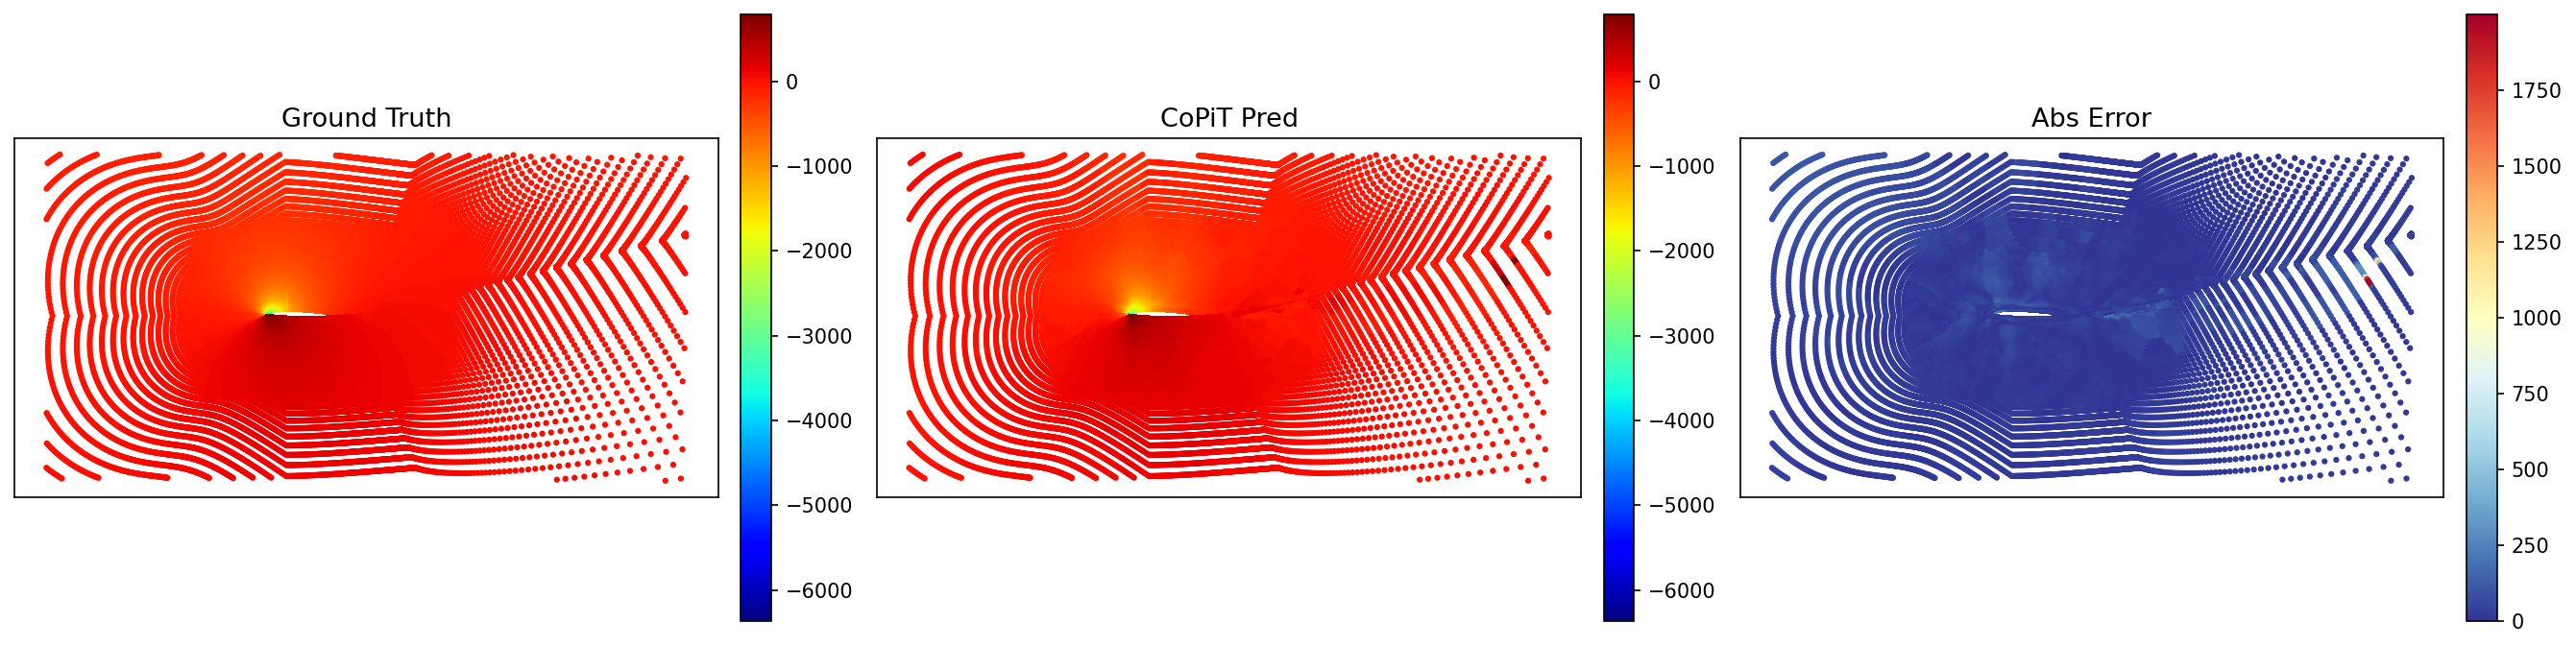
\includegraphics[width=0.98\linewidth,height=0.28\textheight,keepaspectratio]{figs/airfrans_ff_p.png}
  \caption{Full field}
\end{subfigure}\\[0.6em]
\begin{subfigure}[t]{\linewidth}
  \centering
  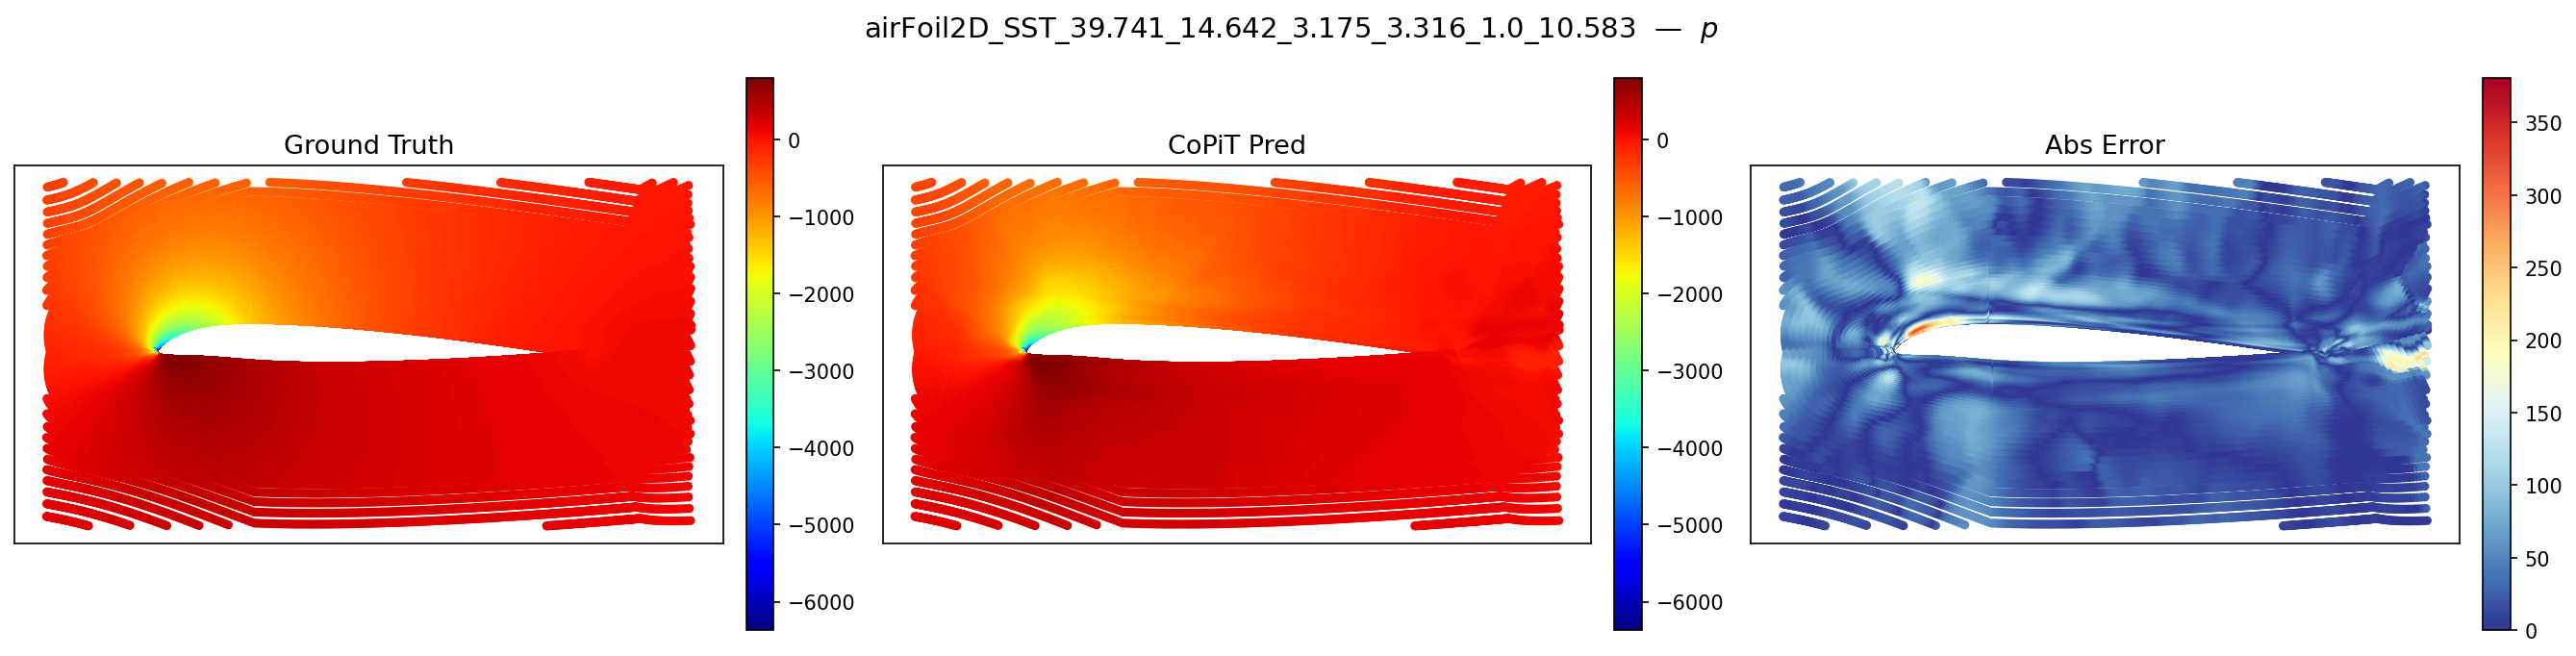
\includegraphics[width=0.98\linewidth,height=0.28\textheight,keepaspectratio]{figs/airfrans_nw_p.png}
  \caption{Near-wall view}
\end{subfigure}
\caption{AirfRANS pressure field on a representative full-data test case: CFD reference, CoPiT prediction and absolute error (full field and near-wall zoom).}
\label{fig:pred_true}
\end{figure}

Since $C_{d}$ and $C_{l}$ are obtained by surface integration of pressure and wall shear, Figure~\ref{fig:airfrans_surf_cmp} compares these surface quantities for CoPiT and Transolver on the same test airfoil. Wall shear is computed from the predicted velocity field under a no-slip wall condition. On this sample CoPiT recovers both the surface pressure and the skin-friction distribution more closely (relative $L^{1}$ pressure error of order $0.06$ versus $0.18$), in line with the improved drag ranking reported below.

\begin{figure}[H]
\centering
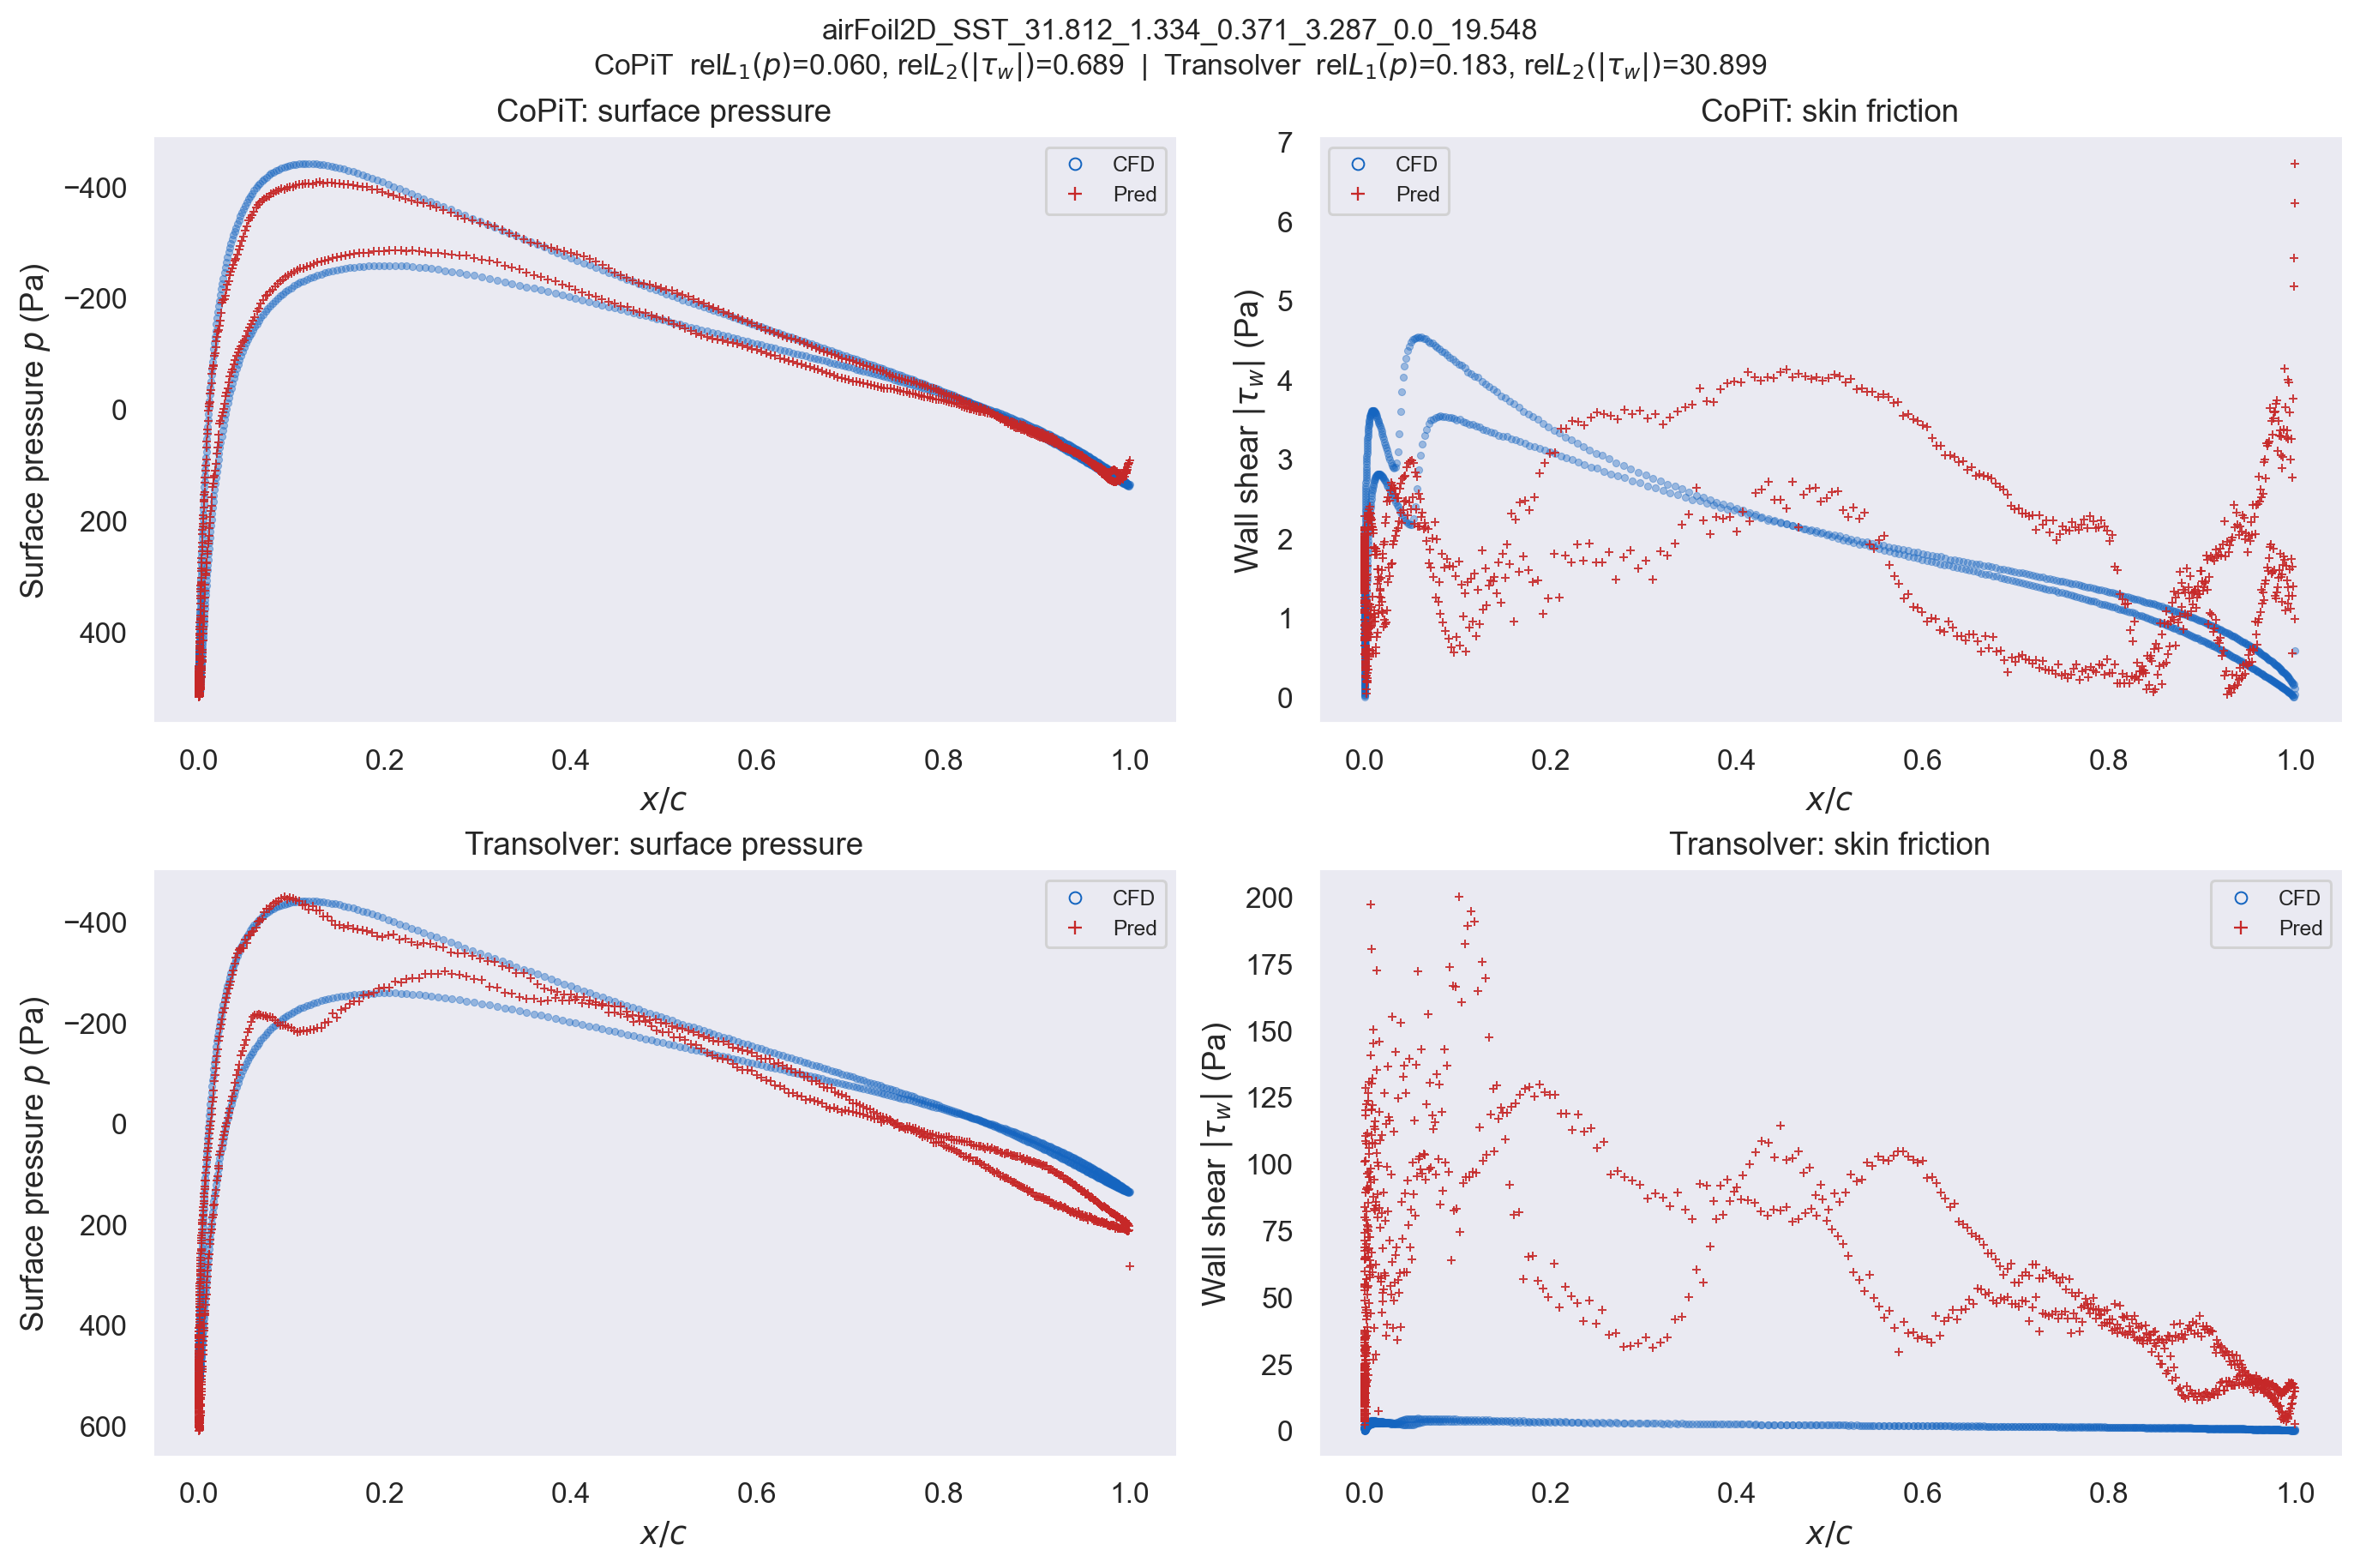
\includegraphics[width=0.98\linewidth,height=0.34\textheight,keepaspectratio]{figs/airfrans_copit_vs_transolver_surf.png}
\caption{Surface pressure and wall shear on a representative AirfRANS test case (\texttt{airFoil2D\_SST\_31.812\_\ldots}). Top: CoPiT; bottom: Transolver. Blue: CFD; orange: prediction. Wall shear is evaluated from the predicted velocity with a no-slip wall condition.}
\label{fig:airfrans_surf_cmp}
\end{figure}

Tables~\ref{tab:full}--\ref{tab:aoa} summarise the four AirfRANS protocols. On the full-data task (Table~\ref{tab:full}), CoPiT attains the lowest surface and volume losses and a drag Spearman correlation $\rho_{d}=0.8388$, far above Transolver ($0.1450$) and graph models with near-zero or negative $\rho_{d}$. Lift correlation is near perfect for both CoPiT and Transolver. CoPiT uses about $1.49\times 10^{6}$ parameters, roughly four times fewer than Transolver (Table~\ref{tab:params}).

\begin{table}[H]
\caption{AirfRANS full-data task. Best results in \textbf{bold}.}
\label{tab:full}
\centering\footnotesize
\begin{tabular}{@{}lcccc@{}}
\toprule
Model & Surf.\ Loss$\downarrow$ & Vol.\ Loss$\downarrow$ & $\rho_d$ & $\rho_l$ \\
\midrule
MLP         & 0.001666 & 0.010895 & $-$0.1169 & 0.9129 \\
GraphSAGE   & 0.001351 & 0.013942 & $-$0.3033 & 0.9651 \\
PointNet    & 0.003068 & 0.037884 & $-$0.0220 & 0.9376 \\
Graph U-Net & 0.002159 & 0.023432 & $-$0.1384 & 0.9667 \\
Transolver  & 0.000346 & 0.007096 &    0.1450 & 0.9981 \\
\textbf{CoPiT} & \textbf{0.000147} & \textbf{0.002822} & \textbf{0.8388} & \textbf{0.9994} \\
\bottomrule
\end{tabular}
\end{table}

\begin{table}[H]
\caption{AirfRANS scarce-data task (200 training samples).}
\label{tab:scarce}
\centering\footnotesize
\begin{tabular}{@{}lcccc@{}}
\toprule
Model & Surf.\ Loss$\downarrow$ & Vol.\ Loss$\downarrow$ & $\rho_d$ & $\rho_l$ \\
\midrule
MLP         & 0.002885 & 0.031496 & $-$0.2423 & 0.9235 \\
GraphSAGE   & 0.002002 & 0.034560 & $-$0.1390 & 0.9813 \\
PointNet    & 0.011009 & 0.136081 & $-$0.0501 & 0.9493 \\
Graph U-Net & 0.003218 & 0.045540 & $-$0.0950 & 0.9760 \\
Transolver  & 0.000541 & \textbf{0.013282} & $-$0.0261 & 0.9890 \\
\textbf{CoPiT} & \textbf{0.000499} & 0.016785 & \textbf{0.4250} & \textbf{0.9963} \\
\bottomrule
\end{tabular}
\end{table}

Under scarce data (Table~\ref{tab:scarce}), CoPiT retains the best surface loss and the best force correlations, while Transolver attains a slightly lower volume loss. Under Reynolds extrapolation (Table~\ref{tab:reynolds}), CoPiT is best on all four reported metrics, although $\rho_{d}$ decreases relative to the full-data regime, indicating that drag remains sensitive to viscous extrapolation. Under angle-of-attack extrapolation (Table~\ref{tab:aoa}), surface losses of CoPiT and Transolver are essentially tied; Transolver is slightly better on volume loss and $\rho_{l}$, whereas CoPiT achieves a markedly higher $\rho_{d}$ ($0.7664$ versus $0.0692$). The advantage of multi-stage conditioning is therefore most pronounced in drag ranking.

\begin{table}[H]
\caption{AirfRANS Reynolds-number extrapolation.}
\label{tab:reynolds}
\centering\footnotesize
\begin{tabular}{@{}lcccc@{}}
\toprule
Model & Surf.\ Loss$\downarrow$ & Vol.\ Loss$\downarrow$ & $\rho_d$ & $\rho_l$ \\
\midrule
MLP         & 0.001452 & 0.010673 & $-$0.1465 & 0.6423 \\
GraphSAGE   & 0.001401 & 0.018527 &    0.0130 & 0.9271 \\
PointNet    & 0.001367 & 0.058220 &    0.0062 & 0.8985 \\
Graph U-Net & 0.002180 & 0.027591 &    0.0280 & 0.9045 \\
Transolver  & 0.000305 & 0.005079 &    0.0898 & 0.9477 \\
\textbf{CoPiT} & \textbf{0.000168} & \textbf{0.003031} & \textbf{0.2478} & \textbf{0.9740} \\
\bottomrule
\end{tabular}
\end{table}

\begin{table}[H]
\caption{AirfRANS angle-of-attack extrapolation.}
\label{tab:aoa}
\centering\footnotesize
\begin{tabular}{@{}lcccc@{}}
\toprule
Model & Surf.\ Loss$\downarrow$ & Vol.\ Loss$\downarrow$ & $\rho_d$ & $\rho_l$ \\
\midrule
MLP         & 0.001555 & 0.007920 &    0.0378 & 0.8608 \\
GraphSAGE   & 0.001048 & 0.007839 &    0.0546 & 0.9078 \\
PointNet    & 0.003279 & 0.026690 &    0.1223 & 0.9357 \\
Graph U-Net & 0.001506 & 0.018316 & $-$0.1955 & 0.9344 \\
Transolver  & \textbf{0.000129} & \textbf{0.001961} &    0.0692 & \textbf{0.9957} \\
\textbf{CoPiT} & \textbf{0.000129} & 0.002334 & \textbf{0.7664} & 0.9810 \\
\bottomrule
\end{tabular}
\end{table}

\begin{table}[H]
\caption{Trainable parameter counts.}
\label{tab:params}
\centering\footnotesize
\begin{tabular}{@{}lcccccc@{}}
\toprule
 & MLP & GraphSAGE & PointNet & Graph U-Net & Transolver & CoPiT \\
\midrule
Params & 19{,}988 & 29{,}204 & 75{,}244 & 65{,}820 & 5{,}996{,}868 & 1{,}494{,}538 \\
\bottomrule
\end{tabular}
\end{table}

Figure~\ref{fig:force_scatter} compares true and predicted force coefficients on the full-data test set (200 cases) under the same integration protocol. CoPiT yields $\rho_{d}\approx 0.839$ and $\rho_{l}\approx 0.999$, whereas Transolver reaches $\rho_{d}\approx 0.145$ and $\rho_{l}\approx 0.998$: lift ranking is strong for both models, while drag ranking is substantially improved by CoPiT.

\begin{figure}[H]
\centering
\begin{subfigure}[t]{\linewidth}
  \centering
  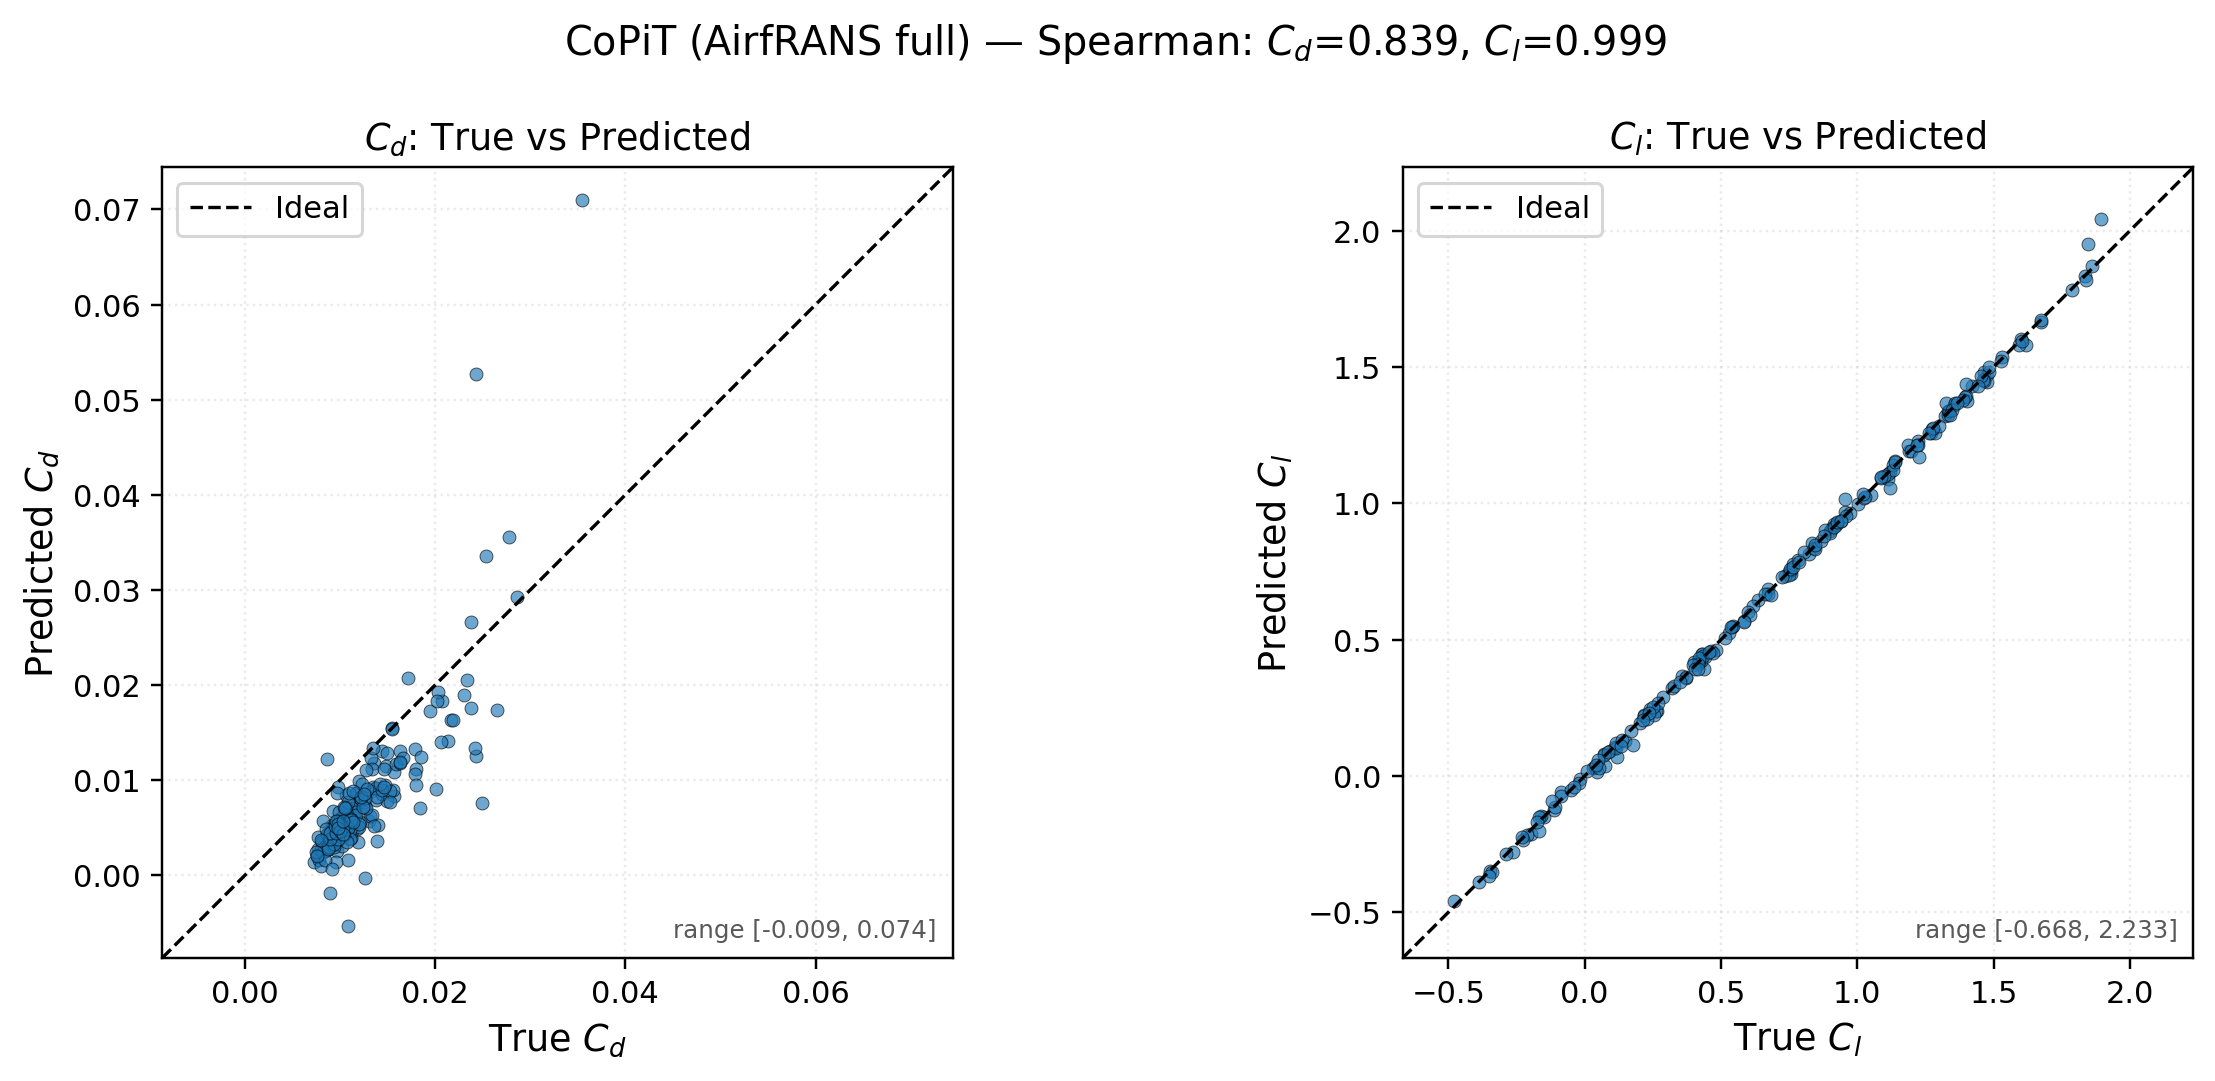
\includegraphics[width=0.92\linewidth,height=0.26\textheight,keepaspectratio]{figs/copit_airfrans_scatter_cd_cl.png}
  \caption{CoPiT}
\end{subfigure}\\[0.6em]
\begin{subfigure}[t]{\linewidth}
  \centering
  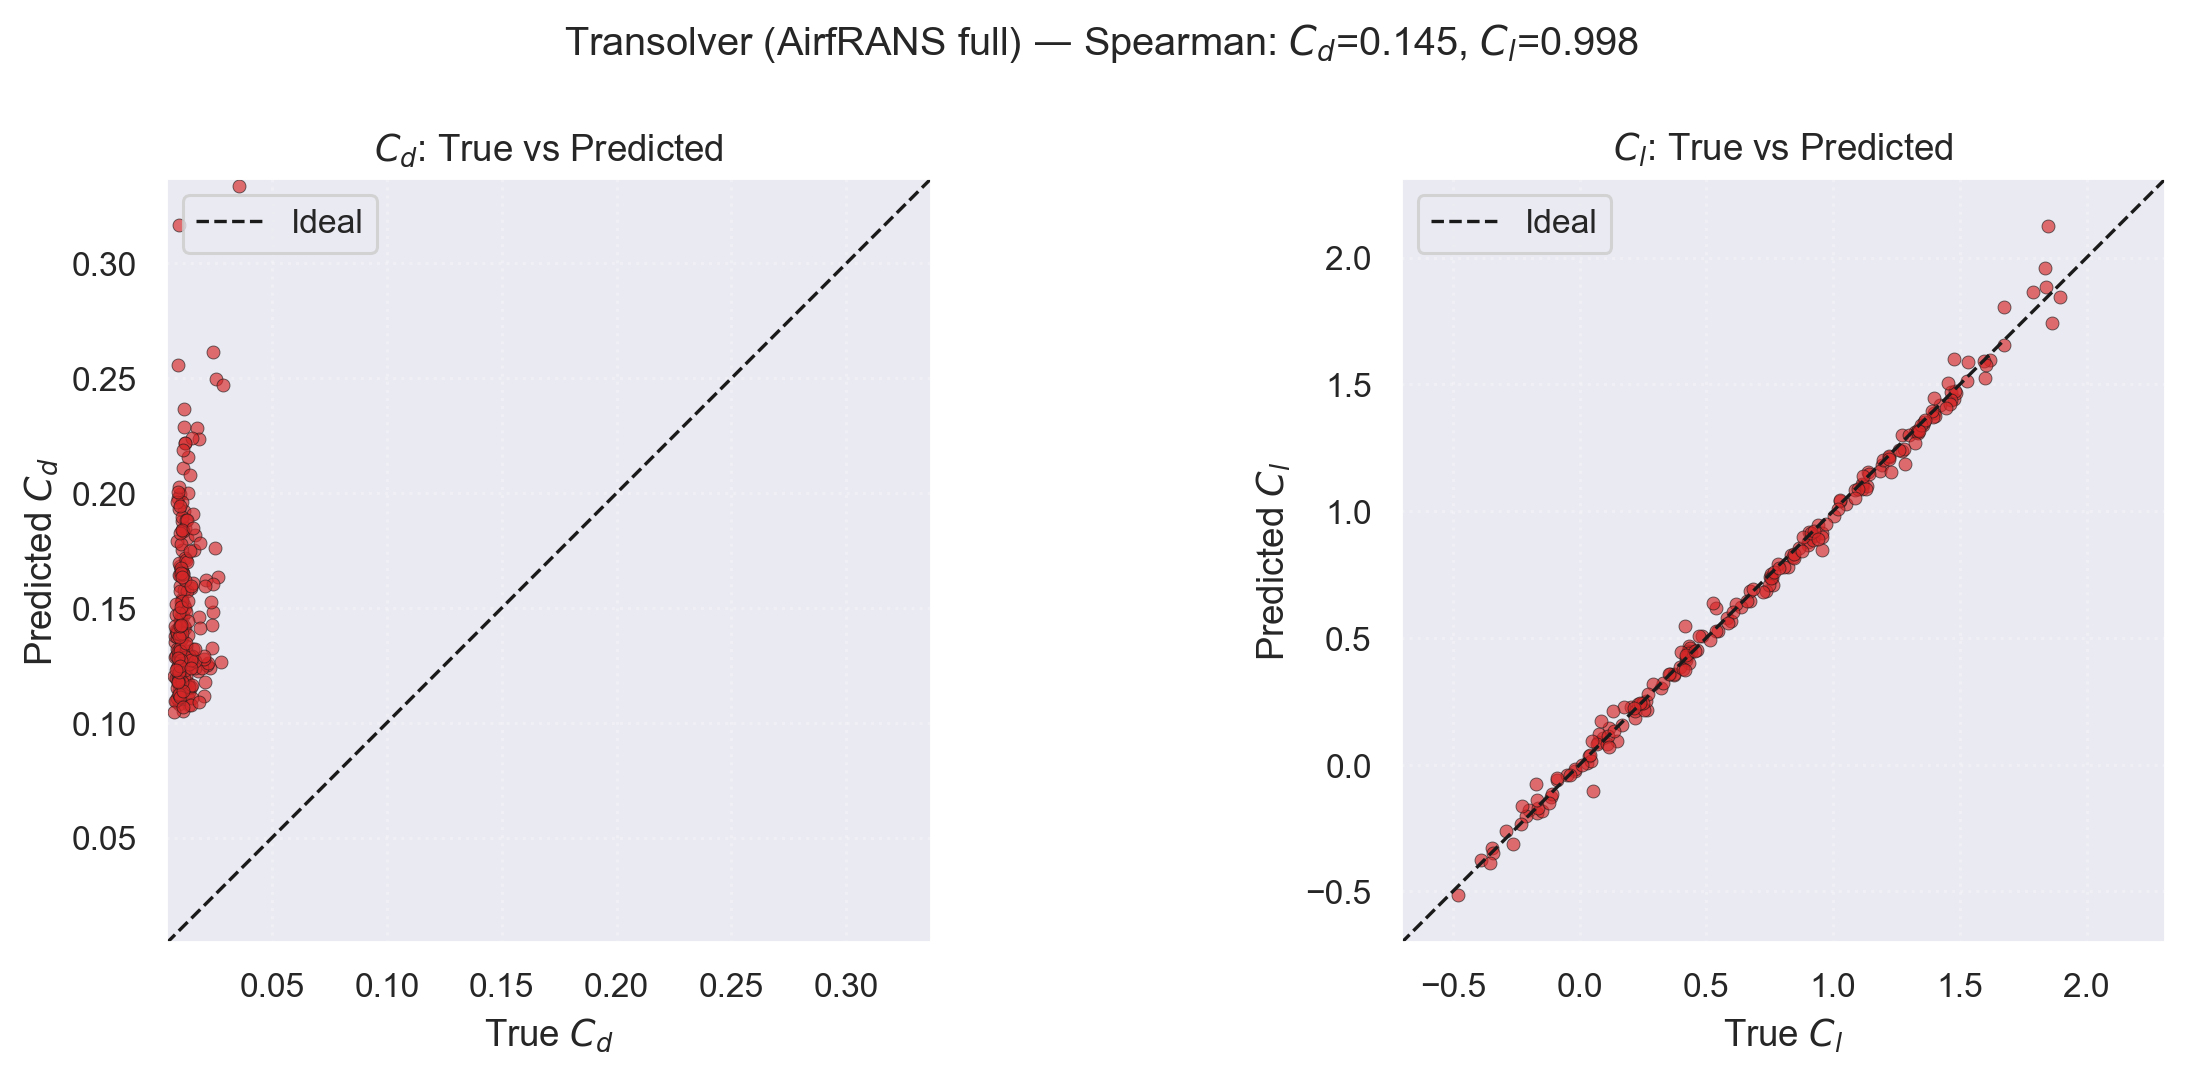
\includegraphics[width=0.92\linewidth,height=0.26\textheight,keepaspectratio]{figs/transolver_airfrans_scatter_cd_cl.png}
  \caption{Transolver}
\end{subfigure}
\caption{True versus predicted $C_d$ (left panels) and $C_l$ (right panels) on the AirfRANS full-data test set.}
\label{fig:force_scatter}
\end{figure}

\subsection{BlendedNet++ results}
\label{sec:blended}

Table~\ref{tab:blendednetpp} reports normalised pointwise MSE on the full test set under the unified reimplementation protocol. CoPiT attains the best overall MSE ($0.0530$) and the best errors on $C_{p}$ and $C_{f,x}$; Transolver is the closest competitor overall ($0.0568$, about $7\%$ higher) and is slightly better on $C_{f,z}$. Streamwise skin friction $C_{f,x}$ is the hardest channel for every model. All scores are expressed in the same per-channel $z$-score space used for training and therefore differ in scale from physical relative errors reported elsewhere.

\begin{table}[H]
\caption{BlendedNet++ forward surface regression under a unified protocol (test set, $N=2{,}498$). Normalised MSE; best in \textbf{bold}.}
\label{tab:blendednetpp}
\centering\footnotesize
\begin{tabular}{@{}lcccc@{}}
\toprule
Model & Overall$\downarrow$ & $C_p$ & $C_{f,x}$ & $C_{f,z}$ \\
\midrule
\textbf{CoPiT} & \textbf{0.0530} & \textbf{0.0181} & \textbf{0.0991} & 0.0417 \\
Transolver  & 0.0568 & 0.0188 & 0.1107 & \textbf{0.0411} \\
FiLMNet     & 0.0691 & 0.0202 & 0.1356 & 0.0516 \\
PointNet    & 0.0715 & 0.0236 & 0.1336 & 0.0572 \\
GraphSAGE   & 0.0859 & 0.0346 & 0.1416 & 0.0817 \\
Graph U-Net & 0.1327 & 0.1320 & 0.1614 & 0.1046 \\
GNOT        & 0.5234 & 0.5055 & 0.5088 & 0.5559 \\
\bottomrule
\end{tabular}
\end{table}

Figure~\ref{fig:blendednetpp_cp_cases} shows a representative test case (\texttt{test\_case\_0674}). Both CoPiT and Transolver recover the large-scale $C_p$ topology; CoPiT exhibits weaker error peaks near the wing--body junction on this sample (surface $C_p$ relative $L^{1}$ error of order $0.06$ versus $0.12$), consistent with the full-test averages in Table~\ref{tab:blendednetpp}.

\begin{figure}[H]
\centering
\begin{subfigure}[t]{0.32\linewidth}
  \centering
  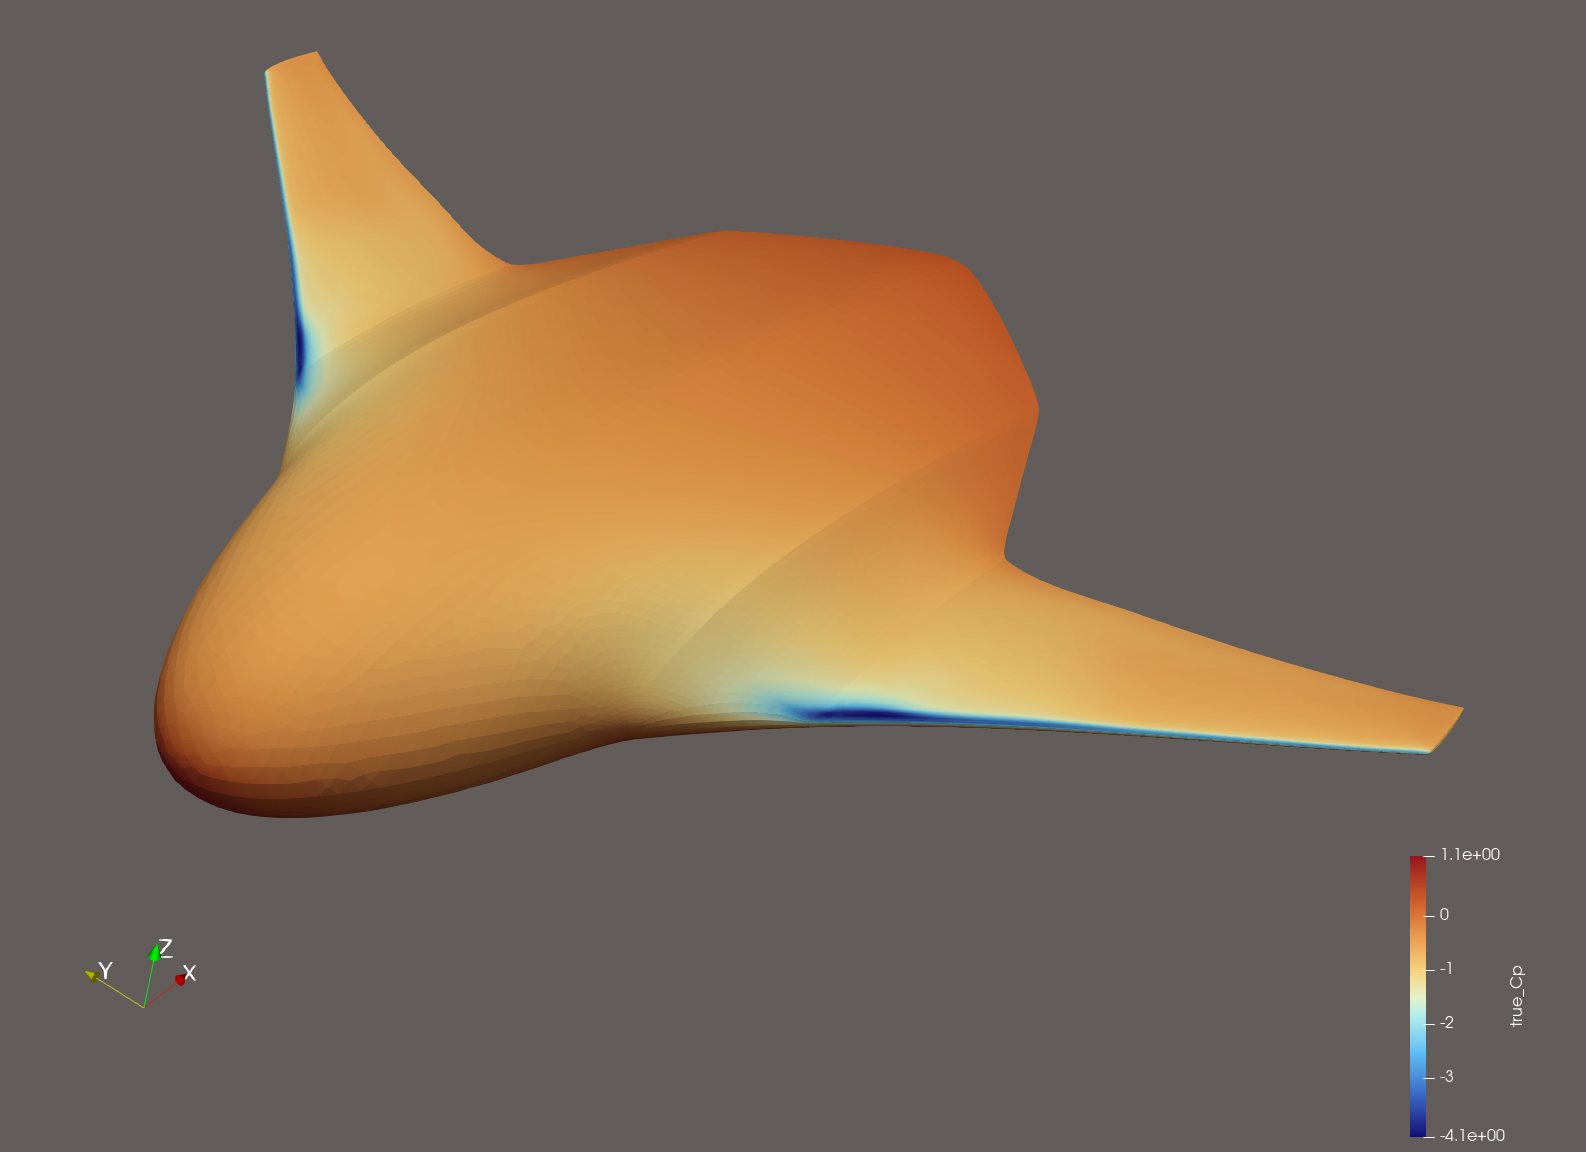
\includegraphics[width=\linewidth,height=0.18\textheight,keepaspectratio]{figs/blend_true.png}
  \caption*{CFD}
\end{subfigure}\hfill
\begin{subfigure}[t]{0.32\linewidth}
  \centering
  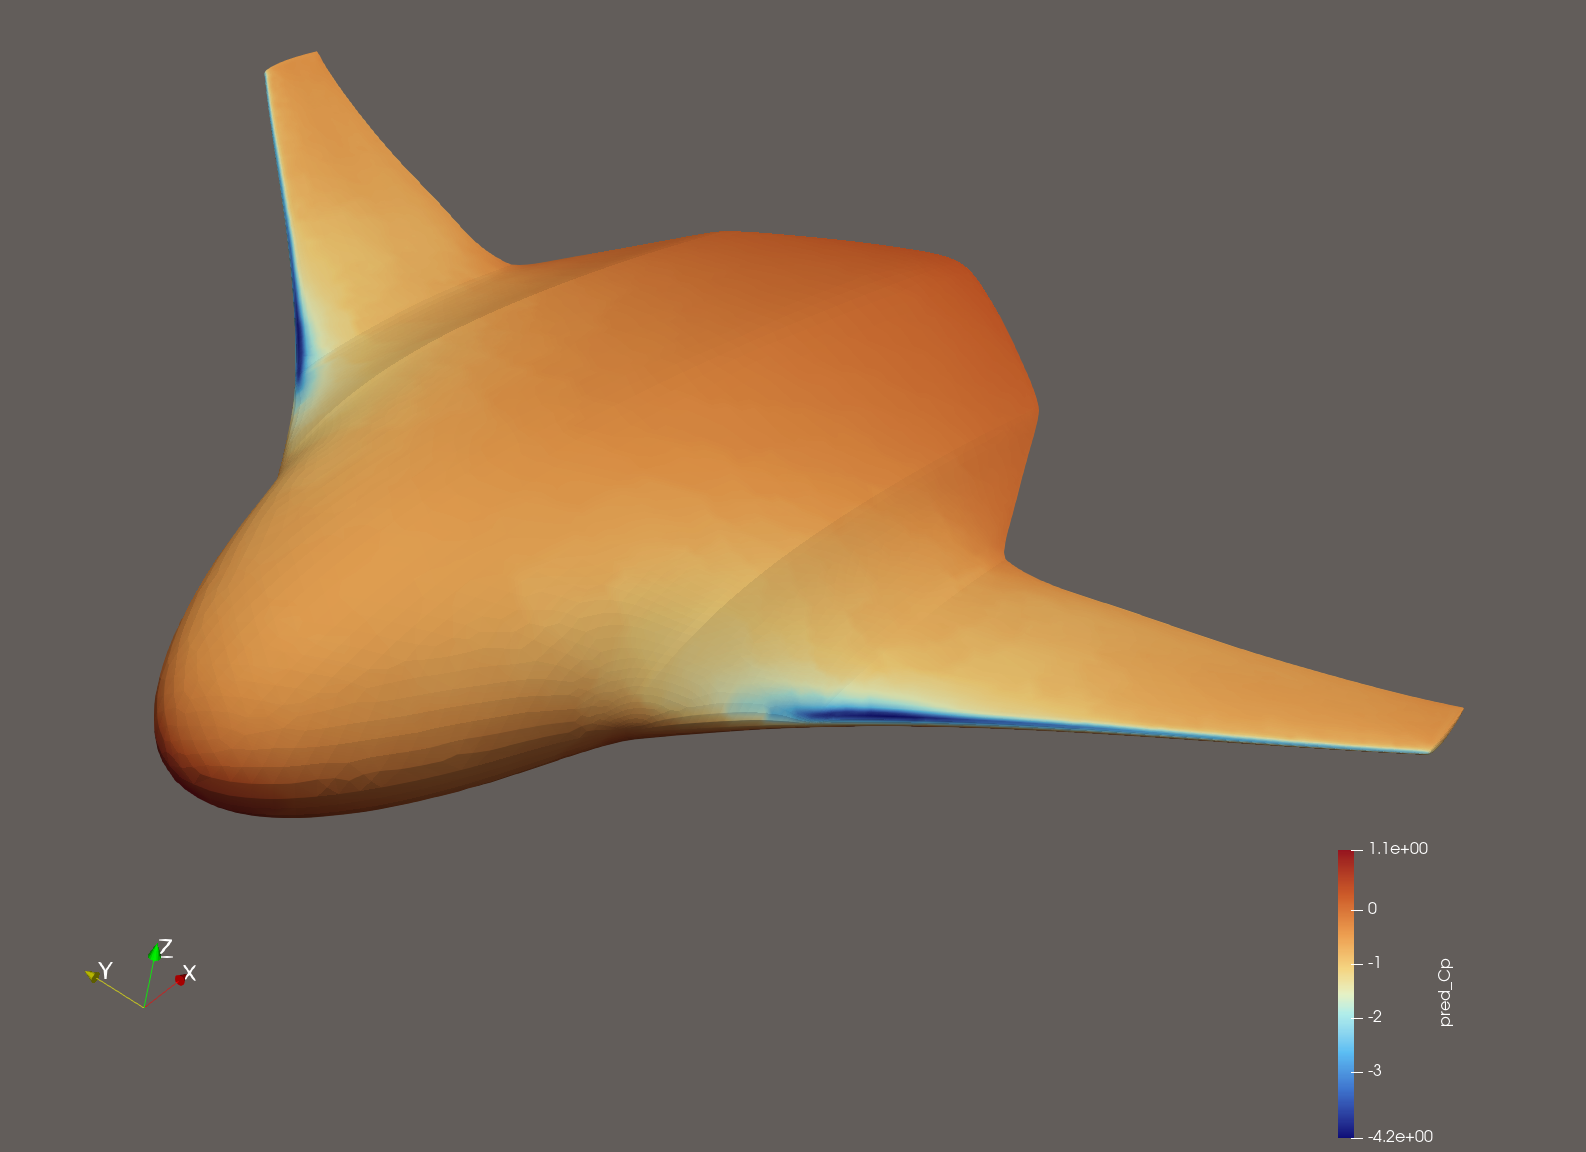
\includegraphics[width=\linewidth,height=0.18\textheight,keepaspectratio]{figs/blend_copit_pred.png}
  \caption*{CoPiT}
\end{subfigure}\hfill
\begin{subfigure}[t]{0.32\linewidth}
  \centering
  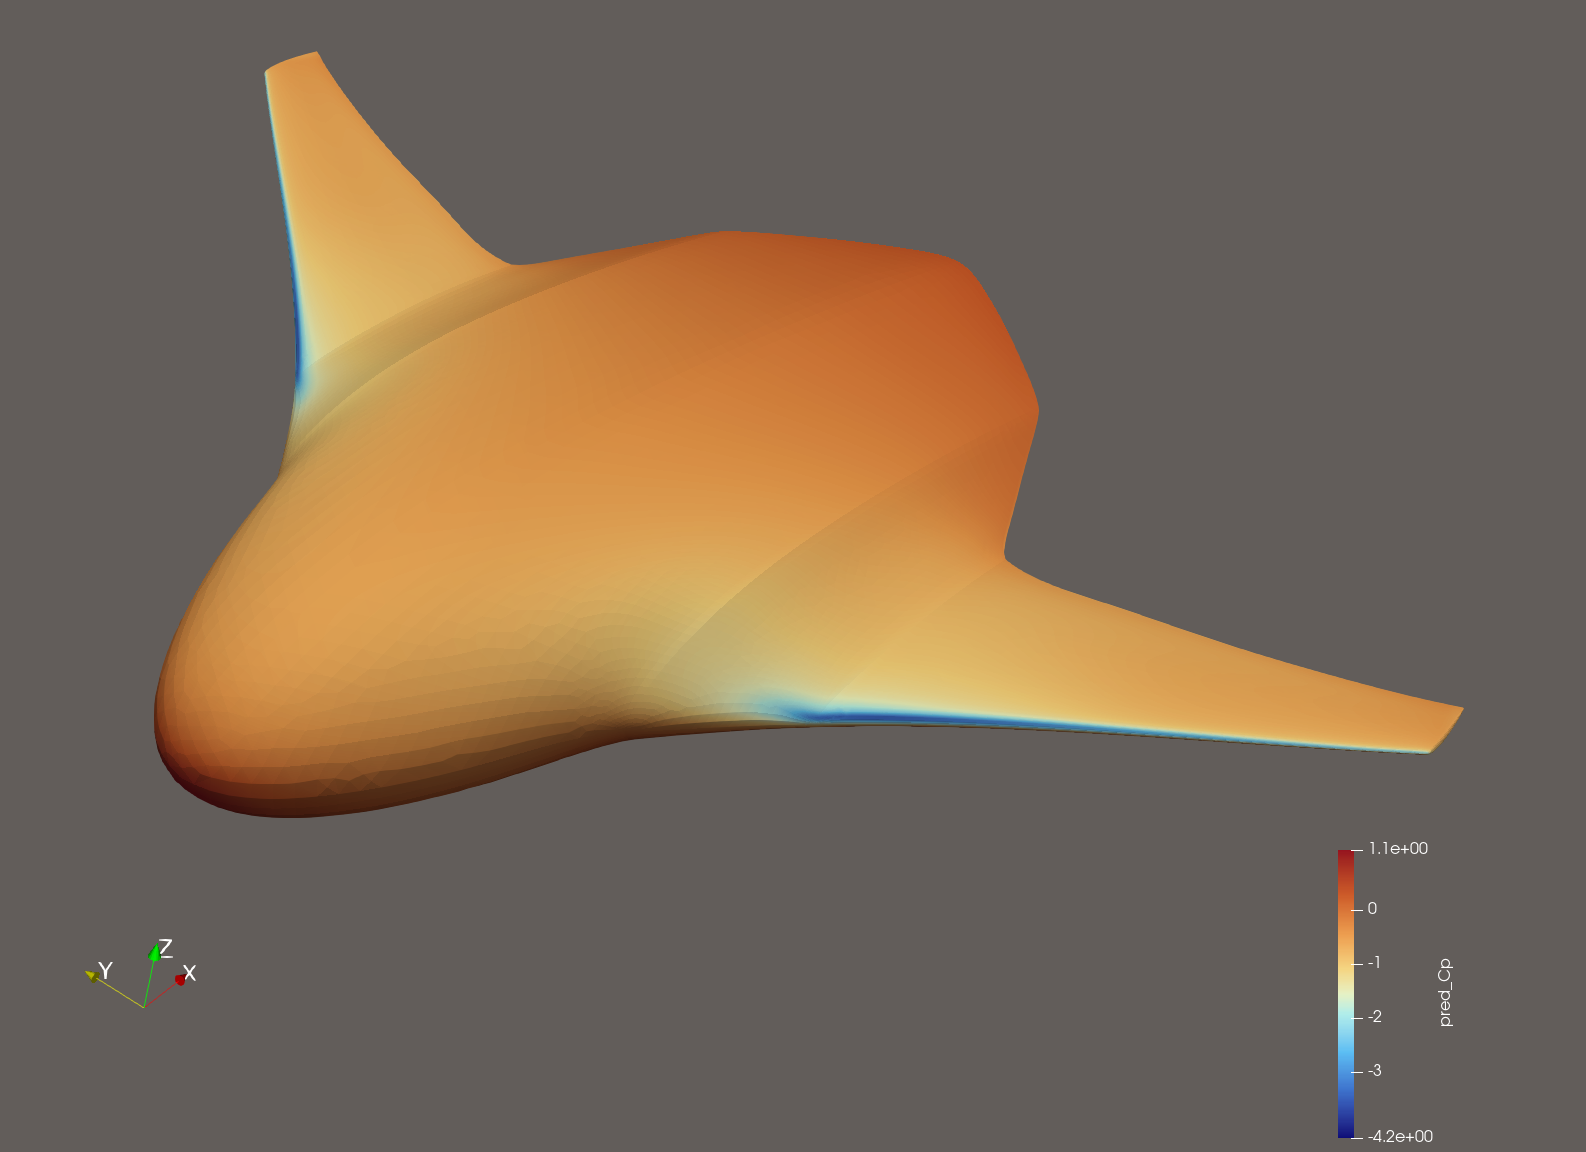
\includegraphics[width=\linewidth,height=0.18\textheight,keepaspectratio]{figs/blend_transolver_pred.png}
  \caption*{Transolver}
\end{subfigure}\\[0.5em]
\begin{subfigure}[t]{0.32\linewidth}
  \centering
  \phantom{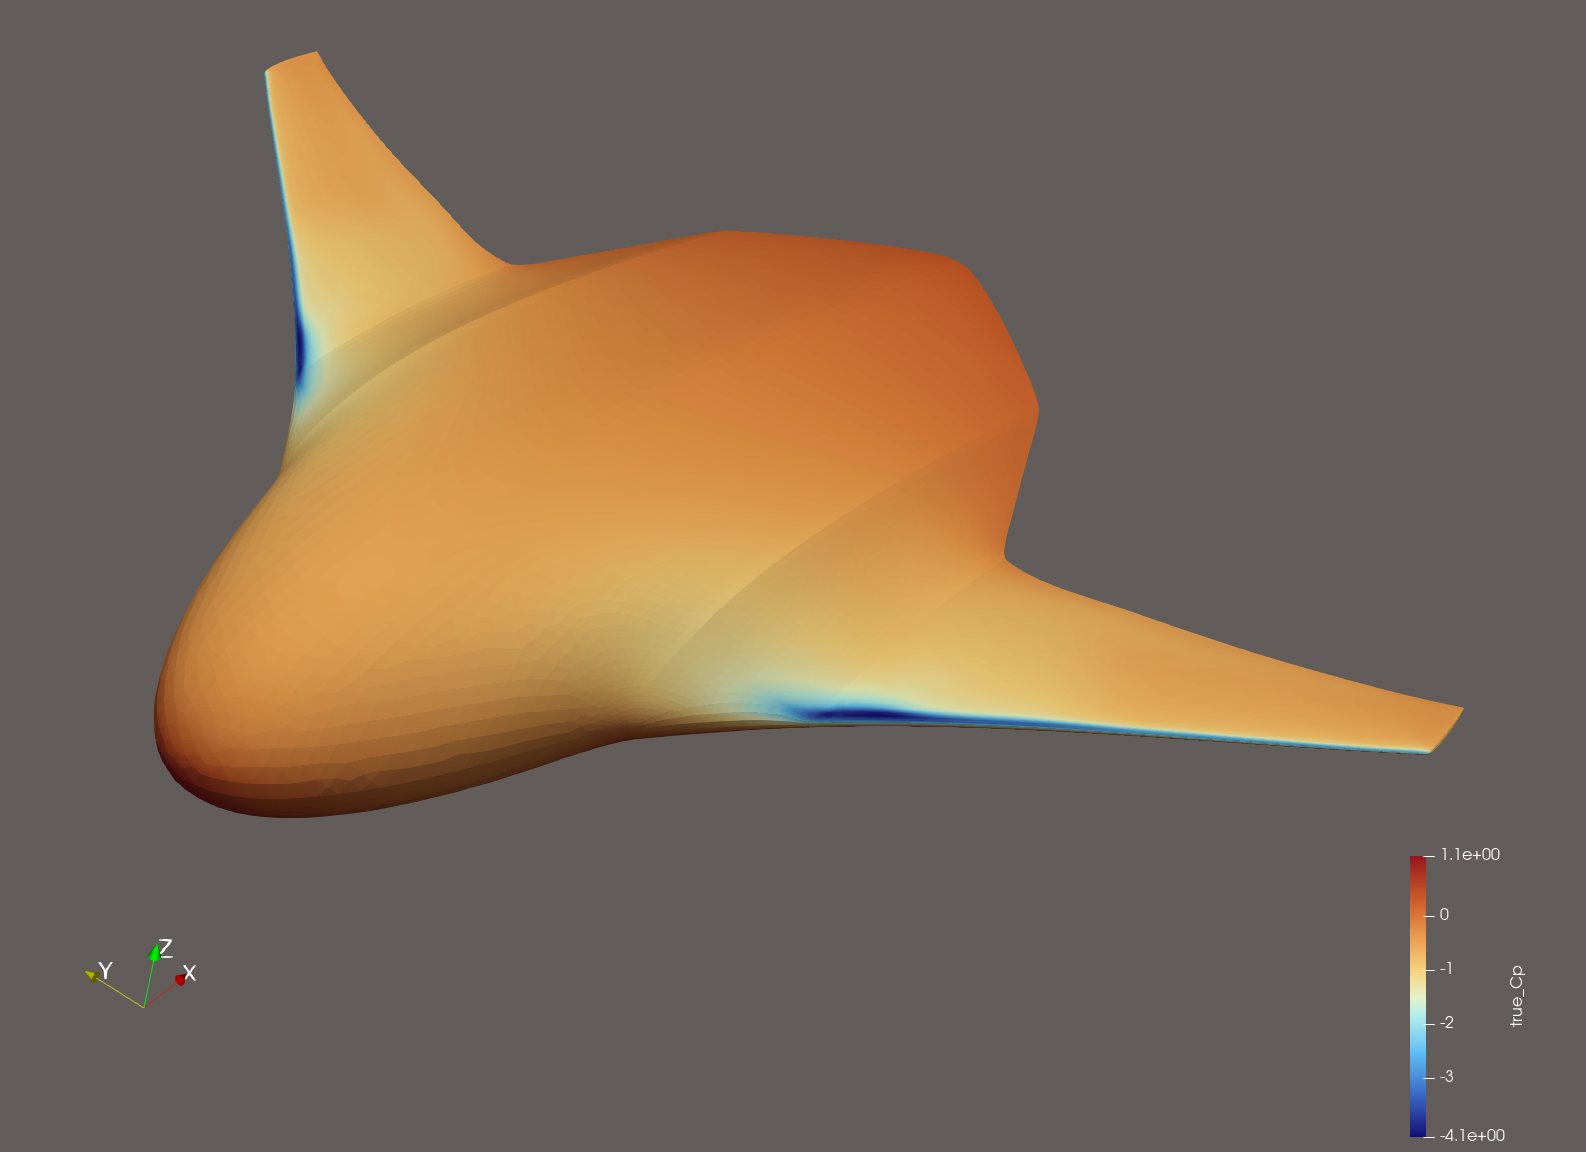
\includegraphics[width=\linewidth,height=0.18\textheight,keepaspectratio]{figs/blend_true.png}}
\end{subfigure}\hfill
\begin{subfigure}[t]{0.32\linewidth}
  \centering
  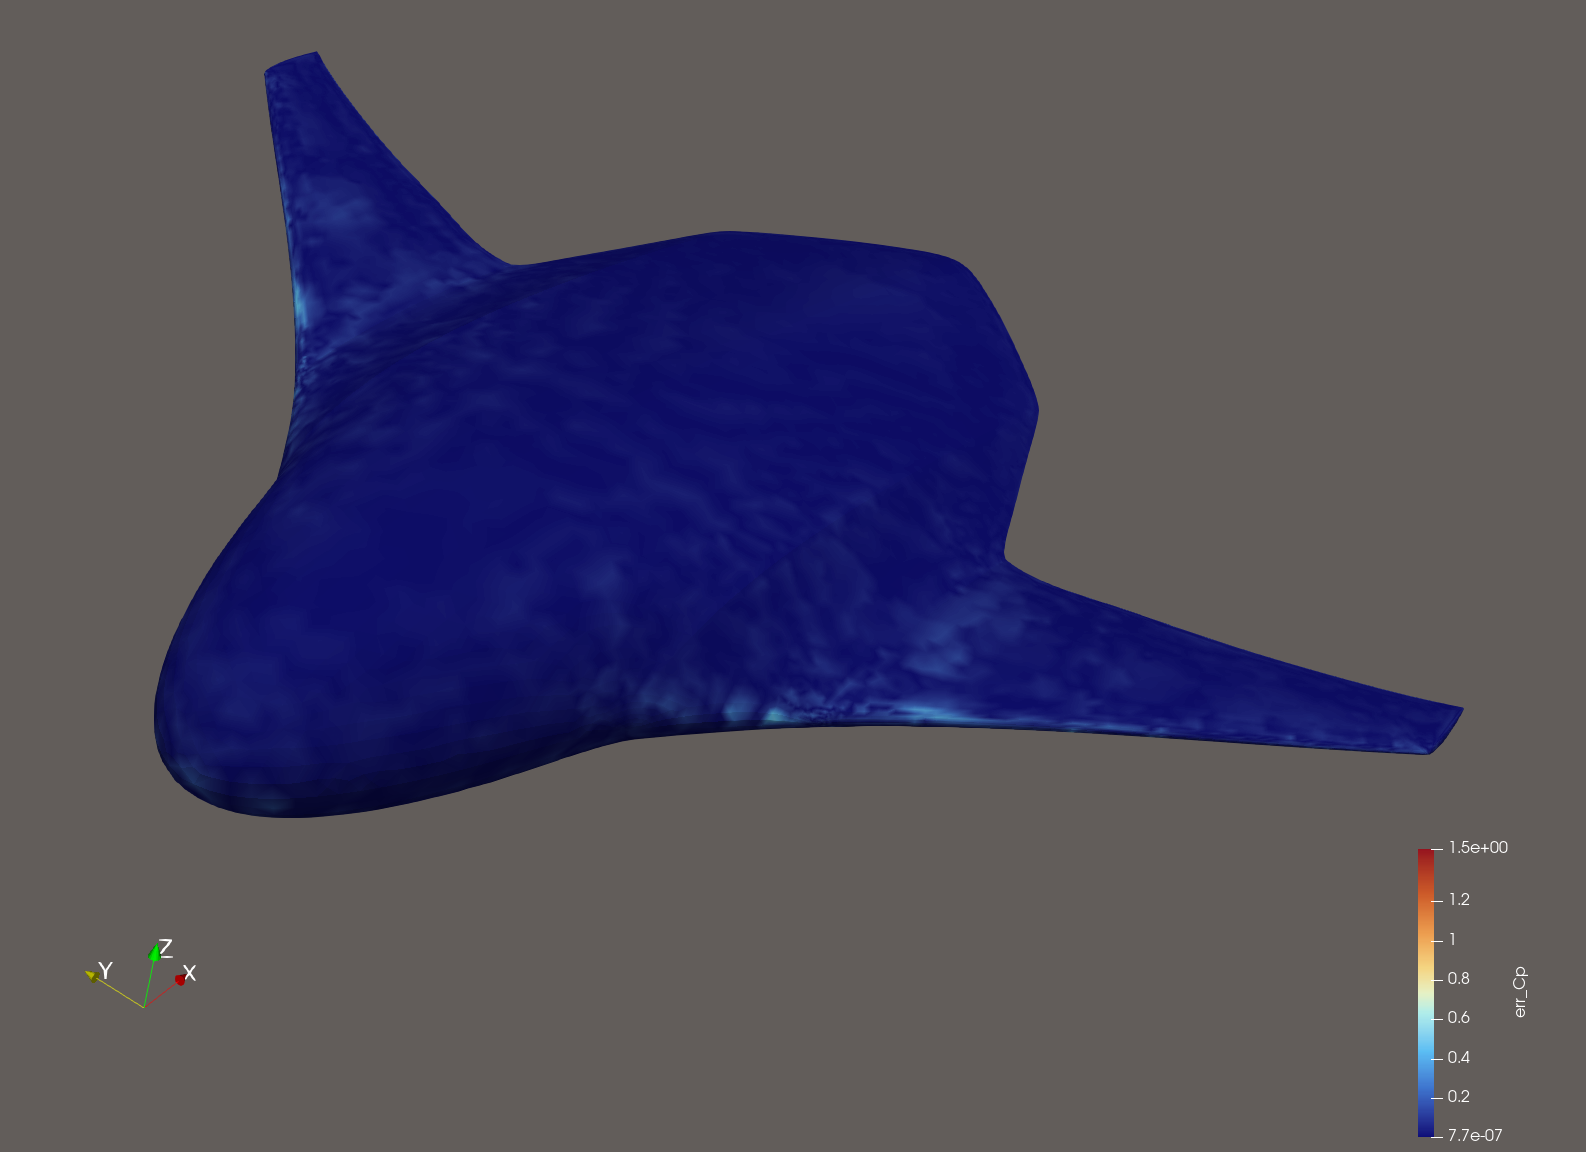
\includegraphics[width=\linewidth,height=0.18\textheight,keepaspectratio]{figs/blend_copit_error.png}
  \caption*{CoPiT error}
\end{subfigure}\hfill
\begin{subfigure}[t]{0.32\linewidth}
  \centering
  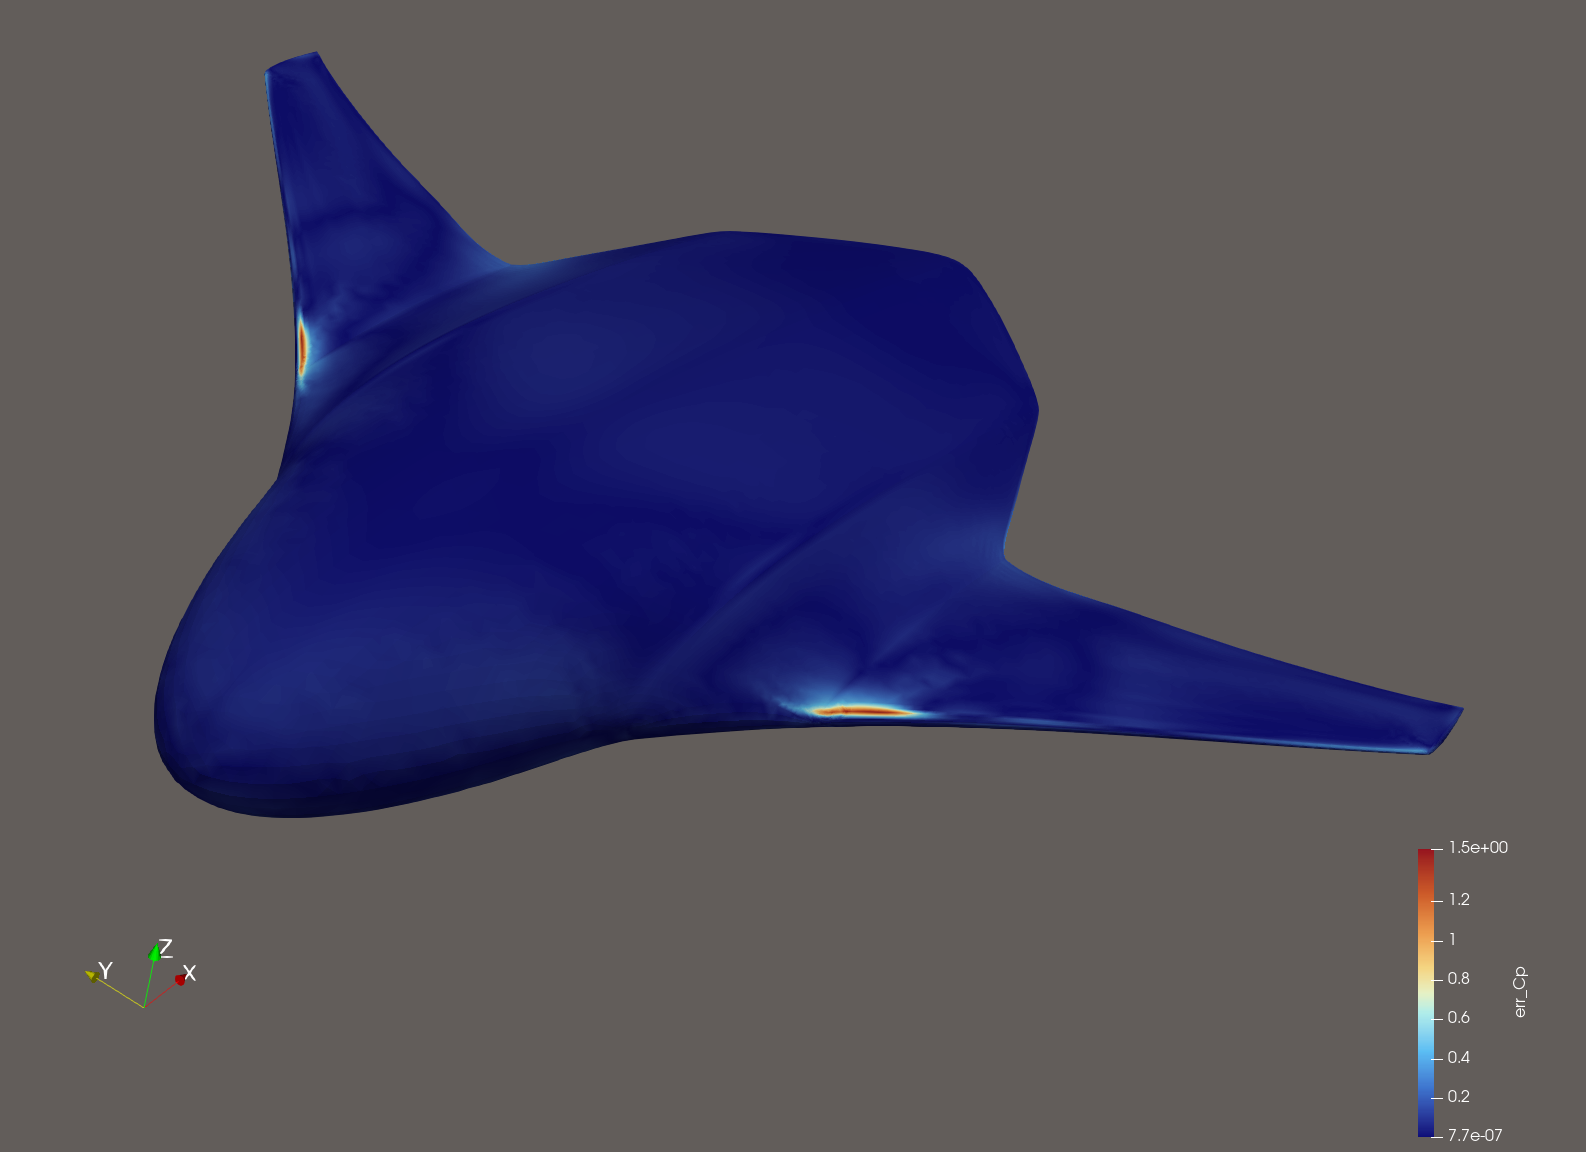
\includegraphics[width=\linewidth,height=0.18\textheight,keepaspectratio]{figs/blend_transolver_error.png}
  \caption*{Transolver error}
\end{subfigure}
\caption{BlendedNet++ surface $C_p$ on \texttt{test\_case\_0674}: CFD reference, CoPiT and Transolver predictions, and absolute errors.}
\label{fig:blendednetpp_cp_cases}
\end{figure}

\subsection{Discussion}
\label{sec:discussion}
\noindent\textbf{Ranking versus absolute error.}\ 
The drag coefficient is a small residual between pressure and friction contributions, so mean relative error is sensitive to modest absolute deviations. Spearman correlation measures the ordering of cases and is often more informative for design screening. Across AirfRANS protocols, CoPiT's clearest advantage is in $\rho_{d}$, consistent with more accurate surface pressure (Figure~\ref{fig:airfrans_surf_cmp}) and with FiLM making the representation more responsive to $(U_{\infty},\alpha)$.

\noindent\textbf{Complexity.}\ 
If $N_{\mathrm{ltt}}$ denotes the latent-mesh size, $L$ the number of processor blocks, $H$ the number of heads and $D$ the hidden width, processor self-attention scales as $\mathcal{O}(L N_{\mathrm{ltt}}^{2} H D)$. Encoder and decoder costs are linear in the full mesh size when locality masking or chunked evaluation is used. The FiLM generators act on a global vector of fixed dimension and contribute a negligible mesh-dependent cost.

\noindent\textbf{Limitations.}\ 
Proximity-based attention may still couple points that are close in ambient space but separated on the surface; geometry-aware metrics reduce this mismatch, while fully topology-aware embeddings remain an open direction. Near-wall residuals dominate the field errors. The present training is fully supervised (surface-weighted or plain MSE); residual-based regularisers and tighter coupling to design optimisation are left for future work.

\section{Conclusion}
\label{sec:conclusion}
%% =====================================================================
We have presented CoPiT, a conditional neural operator for aerodynamic field prediction on irregular meshes. Building on a position-induced Transformer backbone for geometry-aware aggregation, CoPiT injects multi-stage FiLM conditioning from freestream and design parameters in the processor and decoder, thereby separating geometric interaction from parametric modulation while retaining the discretisation consistency of position attention. On AirfRANS, CoPiT improves field accuracy and, more markedly, drag ranking under full, scarce and extrapolation protocols, with fewer parameters than Transolver. On BlendedNet++, under a unified reimplementation of the surface-regression task, CoPiT attains the lowest overall normalised surface MSE among the tested baselines. Future work includes coupling the surrogate to aerodynamic optimisation loops, residual-based or physics-informed losses, adaptive latent meshes and extensions to more complex three-dimensional configurations.

\section*{Declaration of competing interest}
The authors declare that they have no known competing financial interests or personal relationships that could have appeared to influence the work reported in this paper.

\section*{Data availability}
Experiments use the publicly available AirfRANS dataset (\url{https://github.com/Extrality/AirfRANS}) and the BlendedNet++ dataset~\cite{sung2025blendednetpp}. Source code, training scripts, configurations, sample input/output data and checkpoints for the reported tables will be released under the MIT license at \url{https://github.com/<to-be-added>/CoPiT} and archived in the CPC Program Library upon acceptance.

\section*{CRediT authorship contribution statement}
\textbf{Y.\ Fan:} Conceptualization, Methodology, Software, Investigation, Writing -- original draft, Writing -- review \& editing.
%% \textbf{Z.\ Qiao:} Supervision, Writing -- review \& editing.

\FloatBarrier
\bibliographystyle{elsarticle-num}
\bibliography{copit_refs}

\end{document}
